\documentclass{template/openetcs_article}
% Use the option "nocc" if the document is not licensed under Creative Commons
%\documentclass[nocc]{template/openetcs_article}
\usepackage {bsymb,b2latex}
\usepackage{lipsum,url,color}
\graphicspath{{./template/}{.}{./images/}}
\begin{document}
\frontmatter
\project{openETCS}

%Please do not change anything above this line
%============================
% The document metadata is defined below

%assign a report number here
\reportnum{OETCS}

%define your workpackage here
\wp{Work-Package 7: ``Toolchain''}


\newcommand{\true}{\ensuremath{true}}
\newcommand{\btext}[1]{{\it #1}}
\newcommand{\bvar}[1]{\btext{#1}}
\newcommand{\bevent}[1]{\btext{#1}}
\newcommand{\binv}[1]{\btext{#1}}
\newcommand{\bconst}[1]{\btext{#1}}
\newcommand{\bparam}[1]{\btext{#1}}
\newcommand{\bfunc}[1]{\btext{#1}}
\newcommand{\baxiom}[1]{\btext{#1}}
\newcommand{\btype}[1]{\btext{#1}}
\newcommand{\bguard}[1]{\btext{#1}}
\newcommand{\bmachine}[1]{\btext{#1}}
\newcommand{\bctx}[1]{\btext{#1}}

\author{Matthias Güdemann}

\affiliation{Systerel\\
  Les Portes de l’Arbois, Bâtiment A \\
  1090 rue René Descartes \\
  13857 Aix-en-Provence Cedex 3, France
}

\title{Event-B Model of Subset 026, Section 3.13}

% define the coverart
\coverart[width=350pt]{openETCS_EUPL}

\reporttype{Model Description}

%\begin{document}

\maketitle
\tableofcontents
\listoffiguresandtables
\newpage

This document describes a formal model of the requirements of section~3.13 of
the subset 026 of the ETCS specification 3.3.0~\cite{SRS-026-330}. This section
describes the speed and distance monitoring subsystem of ETCS.

The model is expressed in the formal language Event-B~\cite{abrial-eventB-Book}
and developed within the Rodin tool~\cite{rodin-handbook}. This formalism allows
an iterative modeling approach. In general, one starts with a very abstract
description of the basic functionality and step-wise adds additional details
until the desired level of accuracy of the model is reached. Rodin provides the
necessary proof support to ensure the correctness of the refined behavior.

In this document we present an Event-B model of the speed and distance
monitoring subsystem of ETCS. At first, we describe shortly the background of
Event-B, then the overall approach taken to model this section and finally
present the model in detail.

The section~3.13 of the SRS gives a very detailed description of the calculation
of many necessary values for speed and distance monitoring. As Event-B is a
system modeling approach, we give an abstract model of the system. The
calculations are abstracted as functions and the system ensures the correct
parameter flow to the functions. We illustrate the model decomposition
capabilities of Event-B and Rodin by decomposing the overall model into
different functional parts.

For a short introduction on Event-B and the usage of Rodin with models on github
see~\url{https://github.com/openETCS/model-evaluation/blob/master/model/B-Systerel/Event_B/rodin-projects-github.pdf?raw=true}

% \begin{table}[ht]
%   \centering
%   \begin{tabular}[ht]{|l|l|}
%     \hline
%      &  \\
%     \hline
%   \end{tabular}
%   \caption{Glossary}
%   \label{tab:glossary}
% \end{table}

\section{Modeling Strategy}
\label{sec:modeling-strategy}

The section~3.13 of the SRS describes the speed and distance monitoring together
with the necessary parameters and data. The model starts with an abstract
modeling of dataflow of the various intermediate calculated values. This model
is partitioned into functional parts, the model is decomposed using shared
variables and the respective sub-models are refined until the basic calculation
functions are reached.

\section{Model Overview}
\label{sec:model-overview}

The overview of the speed and distance monitoring is shown in
Fig.~\ref{fig:speed-distance-system} from the SRS.

\begin{figure}[ht]
  \centering
  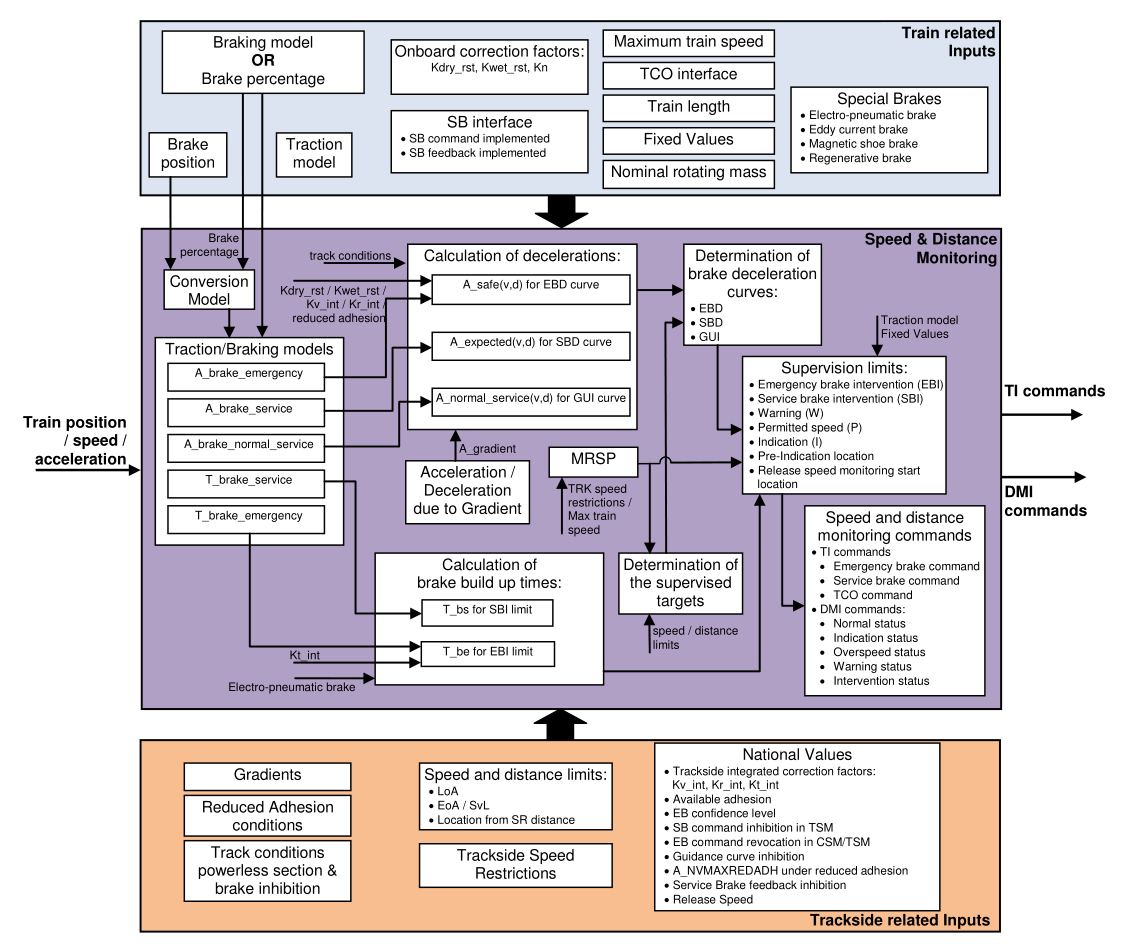
\includegraphics[width=.9\textwidth]{Overview_13_3}
  \caption{Speed and Distance Monitoring Overview~(\cite{SRS-026-330}~p.~85)}
  \label{fig:speed-distance-system}
\end{figure}

The on-board system comprises only the middle layer. The upper layer gives train
related inputs as parameters, the lower layer track related inputs. The system
itself takes the current position, speed and acceleration of the train and
computes commands for the train interface and for the driver machine
interface. For the train interface, this consists of the command for the service
and emergency brakes. For the driver machine interface this consists of the
status indication for the driver.

The Event-B modeling starts with machines describing the dataflow of all inputs,
outputs and intermediate values of the model. For example, the values that are
calculated for \bvar{T\_brake\_service} in \bmachine{Traction / Braking Models}
are written into a variable by an event that calculates then and these values
and are read as input by the event that calculates \bvar{T\_bs} for \bvar{SBI}
limit.

This approach is conducted for each intermediate value of the system until a
single machine is created with one variable for each intermediate value as well
as for each input and output. On this level of modeling, all events only define
the necessary input values and write a new value to their output variable. This
value is provided as event parameter on this abstraction level.

The next step is to decompose the single machine into different sub-machines, in
general one machine for each functional part of the model. This allows for model
structuring and complexity reduction for each machine. For this we use the Rodin
decomposition
plug-in~\footnote{\url{http://wiki.event-b.org/index.php/Decomposition_Plug-in_User_Guide}}
using the shared-variable decomposition
approach~\cite{silva2011decomposition}. This approach splits the set of events
of a machine into several disjoint sets and assigns one such set to each
sub-machine. It also allows to distribute the variables over several machines,
effectively implementing a shared variable distributed system.

The borders for the subsystem decomposition are shown in
Fig.~\ref{fig:system-decomposition}. The dashed lines show the separate
sub-machines. The dataflows that cross these lines are represented by the shared
variables of the decomposed model.

\begin{figure}[ht]
  \centering
  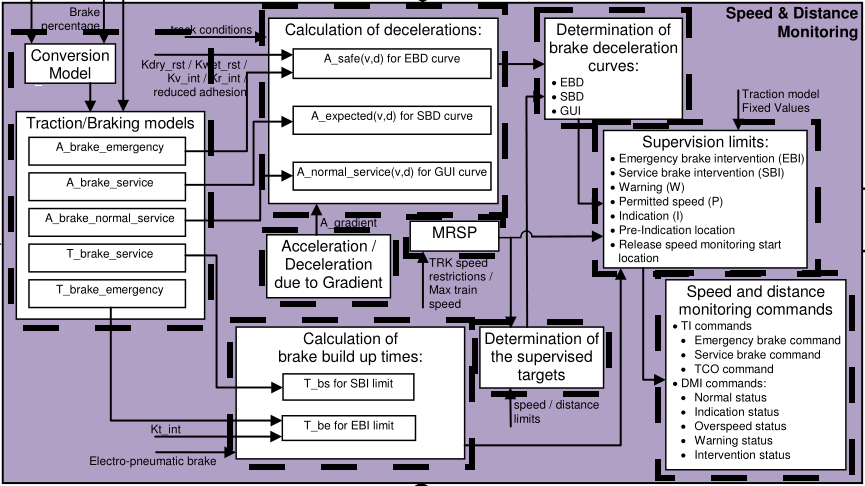
\includegraphics[width=.66\textwidth]{OverviewSelected}
  \caption{Decomposition of System}
  \label{fig:system-decomposition}
\end{figure}

Each of the sub-machines with its shared variables is then further refined until
the desired level of detail is reached. The overview of these refinements is
shown in Fig.~\ref{fig:machine-decompositon-overview}.

\begin{figure}[ht]
  \centering
  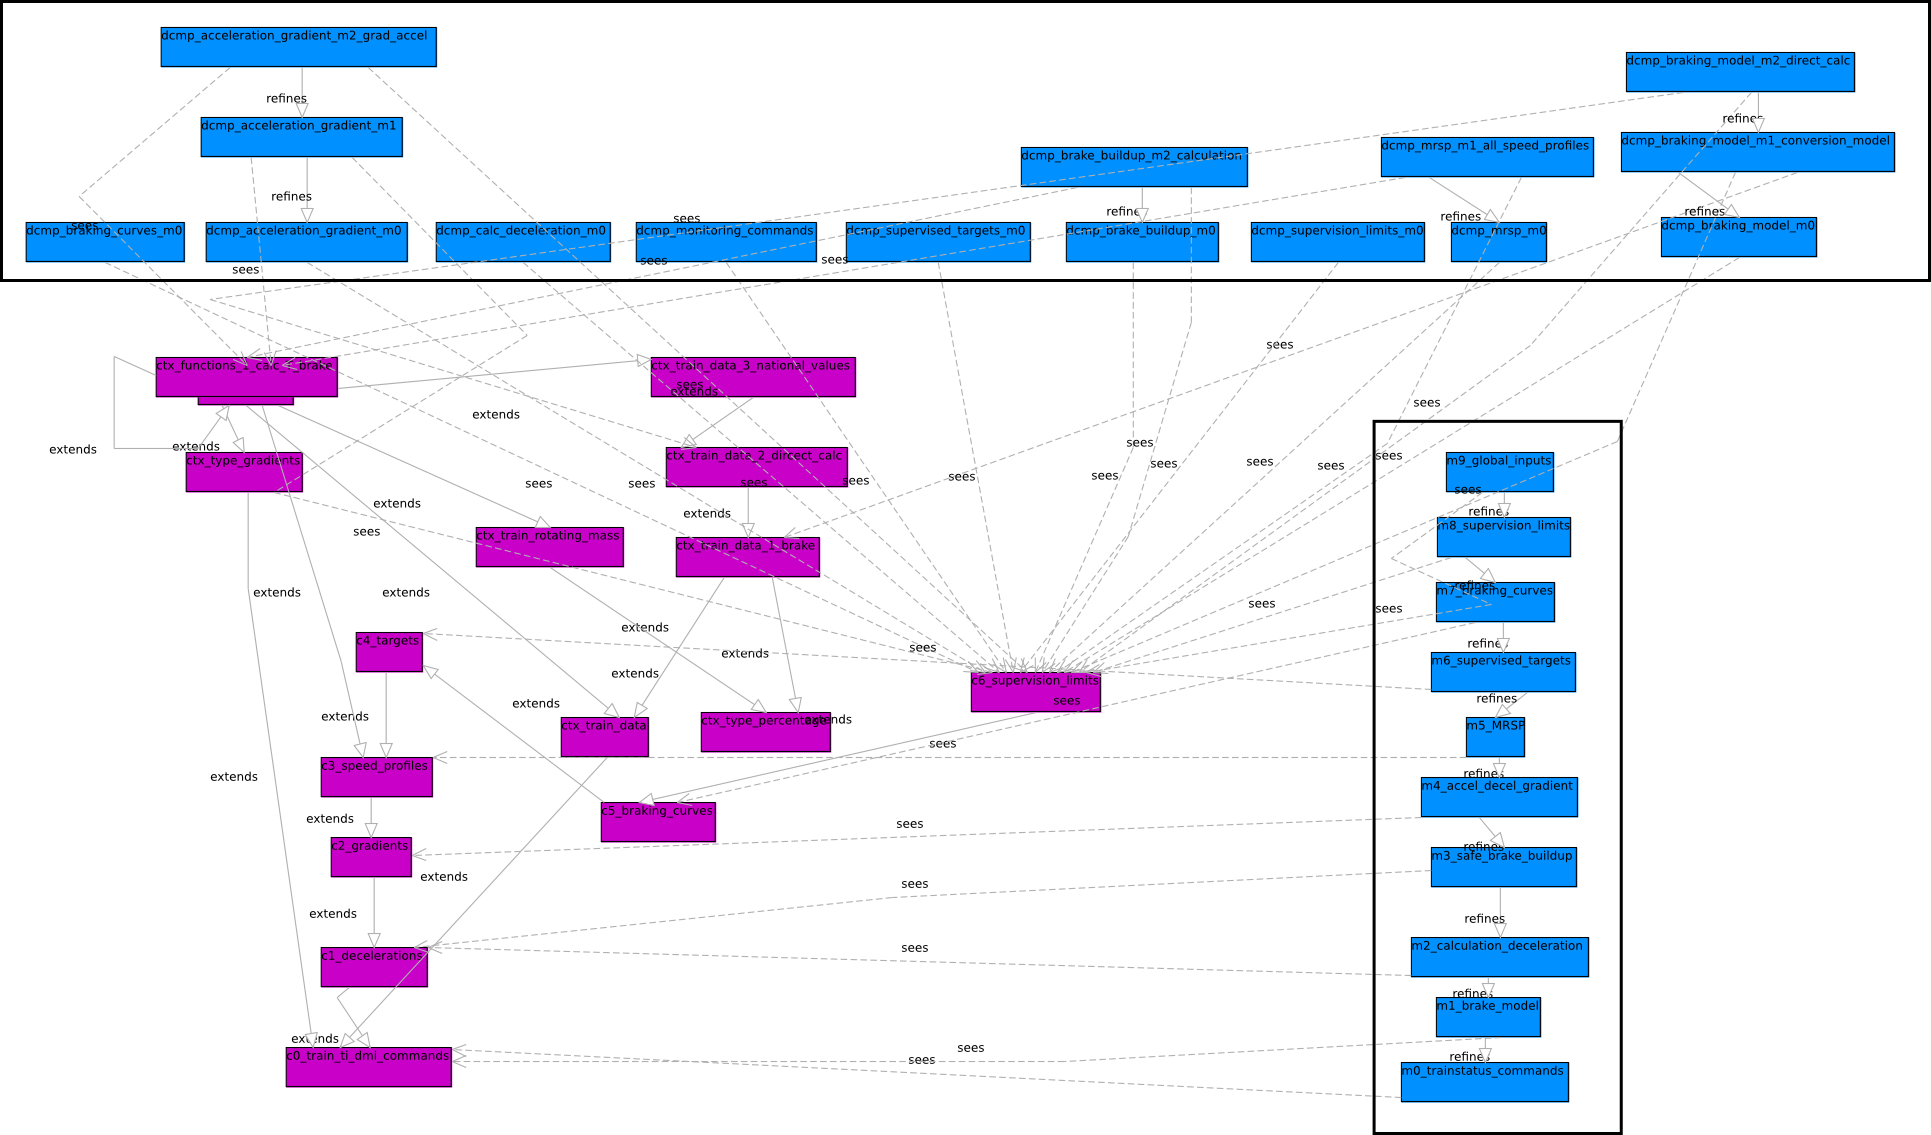
\includegraphics[width=\textwidth]{Section_3_13-layout}
  \caption{Machine Decomposition Overview}
  \label{fig:machine-decompositon-overview}
\end{figure}

This refinement and context overview is very different from the others, as first
an abstract global model was developed and then this model was decomposed into
sub-models which are further refined. The contexts are shared between the
decomposed models as far as possible. In this case, all resulting contexts and
machines are kept in the same Rodin project. It is also possible to create
a new project for each sub-machine which will reduce the complexity of each
single project.

The global model is shown in the lower right. The first machine describes the
global input and output variables of the system. The further refinements
represent the iterative addition of more functions as shown in
Fig.~\ref{fig:system-decomposition}. For example the machine 1 adds the brake
model with its inputs and outputs and the machine 2 adds the calculation of
deceleration which uses the outputs of the braking model.

The last machine is then decomposed into the nine machines representing each a
single functional block. This structure is shown in the upper part of
Fig.~\ref{fig:machine-decompositon-overview}, this also illustrates the further
independent refinement of the decomposed sub-machine.

The context hierarchy also reflects this structuring. The contexts define the
data types for the intermediate values, as well as the functions that calculate
these values. These functions are generally not further refined in the Event-B
model, as this is not part of the system modeling.

\section{Model Benefits}
\label{sec:model-highlights}

The modeled section of the SRS provides many details for calculation of various
values. The main content from a system modeling point of view is the model. So
while in this case the same benefits from using Rodin as
for~\cite{Section-3-5-Rodin,Section-4-6-Rodin,Section-5-9-Rodin} are present,
the main advantage here is the model structuring facility.

\begin{itemize}
\item {\bf Model Decomposition} The shared variable model
  decomposition~\cite{silva2011decomposition} allows for decomposing an Event-B
  model and for separate refining of the machines of the resulting
  sub-models while retaining correctness of the refinement proofs.
\end{itemize}

It should be noted that this section contains mainly very specific
implementation details and no general requirements. Currently, the proof support
for non-linear arithmetic (in particular for floating point numbers) is limited
in Rodin, so the modeling contains mainly the system level. It describes in
particular the decomposition of the model, the various inputs and outputs of the
different model components and the refinement stops when the functional level is
reached. This means that for calculations, the last refinement level in general
describes a function with the required input and output value and correct types.

\section{Detailed Model Description}
\label{sec:deta-model-descr}


\subsection{Context 0 - Train Inputs, TI and DMI command}
\label{sec:context-0-entities}

The first context introduces many basic type for the model,
\btype{t\_locations}, \btype{t\_speed}, \btype{t\_acceleration},
\btype{t\_TI\_commands}, \btype{t\_DMI\_commands}, \btype{t\_time} and
\btype{t\_train\_modes}.

The commands for the train interface (TI) are represented by the constants
\bconst{c\_emergency\_brake}, \bconst{c\_service\_brake}, \bconst{c\_TCO},
\bconst{c\_no\_command}. For the driver machine interface (DMI) the commands are
represented by the constants \bconst{c\_normal}, \bconst{c\_indication},
\bconst{c\_overspeed}, \bconst{c\_warning} and \bconst{c\_intervention}.

The other constants provide default values for the initialization of variables
of that type.

{\footnotesize
\begin{description}
\CONTEXT{c0\_train\_ti\_dmi\_commands}
\SETS
        \begin{description}
                \ItemY{ t\_locations }{all possible locations on track }
                \ItemY{ t\_speed }{train speed measurement }
                \ItemY{ t\_acceleration }{train acceleration }
                \ItemY{ t\_TI\_commands }{track interface commands }
                \ItemY{ t\_DMI\_commands }{driver machine interface commands }
                \ItemY{ t\_time }{ }
                \Item{ t\_train\_modes }
        \end{description}
\CONSTANTS
        \begin{description}
                \Item{ c\_emergency\_brake }
                \Item{ c\_service\_brake }
                \ItemY{ c\_TCO }{traction cut off}
                \ItemY{ c\_no\_command }{empty command}
                \Item{ c\_normal }
                \Item{ c\_indication }
                \ItemY{ c\_overspeed }{}
                \ItemY{ c\_warning }{}
                \ItemY{ c\_intervention }{}
                \Item{ c\_v0 }
                \Item{ c\_a0 }
                \ItemY{ c\_l0 }{}
                \Item{ c\_a\_brake0 }
                \ItemY{ c\_T\_brake0 }{}
        \end{description}
\AXIOMS
        \begin{description}
                \nItem{ axm1 }{ partition(t\_TI\_commands,\{ c\_no\_command\}
                  ,\{ c\_emergency\_brake\} ,\\ \hspace*{1.2cm} \{ c\_service\_brake\} ,\{ c\_TCO\} ) }\cmt{ }
                \nItem{ axm2 }{ partition(t\_DMI\_commands,\{ c\_normal\} ,\{
                  c\_indication\},\\ \hspace*{1.2cm}\{ c\_overspeed\} ,\{ c\_warning\} ,\{ c\_intervention\} ) }		\nItem{ axm3 }{ c\_v0 \in  t\_speed }		\nItem{ axm4 }{ c\_a0 \in  t\_acceleration }\cmt{ }
                \nItem{ axm5 }{ c\_l0 \in  t\_locations }		\nItem{ axm6 }{ c\_a\_brake0 \in  t\_speed \tfun  t\_acceleration }\cmt{		\\\hspace*{1,4 cm}  default brake profile }
                \nItem{ axm7 }{ c\_T\_brake0 \in  t\_time }\cmt{		\\\hspace*{1,4 cm}  default brake buildup time }
        \end{description}
\END
\end{description}

}

\subsection{Machine 0 - Train Status and Commands}
\label{sec:machine-0-train}

This first machine introduces the external input variables, i.e., the position,
speed and acceleration of the train as well as the output variables, i.e., the
TI commands and the DMI commands. The input variables are read by the event
\bevent{update\_train\_style} and the output variables by the event
\bevent{new\_outputs}.

{\footnotesize
\begin{description}
\MACHINE{m0\_trainstatus\_commands}
\SEES{c0\_train\_ti\_dmi\_commands}
\VARIABLES
        \begin{description}
                \ItemY{ v\_current }{current speed of train}
                \ItemY{ a\_current }{current acceleration of train}
                \ItemY{ loc\_current }{current position of train as track location}
                \ItemY{ cmd\_current }{current TI command}
                \ItemY{ status\_current }{current DMI status}
        \end{description}
\INVARIANTS
        \begin{description}
                \nItem{ inv1 }{ v\_current \in  t\_speed }
                \nItem{ inv2 }{ a\_current \in  t\_acceleration }
                \nItemY{ inv3 }{ loc\_current \in  t\_locations }{  }
                \nItem{ inv4 }{ cmd\_current \in  t\_TI\_commands }
                \nItemY{ inv5 }{ status\_current \in  t\_DMI\_commands }{  }
        \end{description}
\EVENTS
        \INITIALISATION
                \begin{description}
                \BeginAct
                        \begin{description}
                        \nItem{ act1 }{ v\_current :=  c\_v0 }
                        \nItem{ act2 }{ a\_current :=  c\_a0 }
                        \nItemY{ act3 }{ loc\_current :=  c\_l0 }{  }
                        \nItemY{ act4 }{ cmd\_current :=  c\_no\_command }{  }
                        \nItemY{ act5 }{ status\_current :=  c\_normal }{  }
                        \end{description}
                \EndAct
                \end{description}
        \EVT {update\_train\_state}
                \begin{description}
                \AnyPrm
                        \begin{description}
                        \Item{l\_speed }
                        \Item{l\_accel }
                        \Item{l\_loc }
                        \end{description}
                \WhereGrd
                        \begin{description}
                        \nItem{ grd1 }{ l\_speed \in  t\_speed }
                        \nItem{ grd2 }{ l\_accel \in  t\_acceleration }
                        \nItemY{ grd3 }{ l\_loc \in  t\_locations }{ }
                        \end{description}
                \ThenAct
                        \begin{description}
                        \nItem{ act1 }{ v\_current :=  l\_speed }
                        \nItem{ act2 }{ a\_current :=  l\_accel }
                        \nItem{ act3 }{ loc\_current :=  l\_loc }
                        \end{description}
                \EndAct
                \end{description}
        \EVT {new\_outputs}
                \begin{description}
                \AnyPrm
                        \begin{description}
                        \Item{l\_ti\_cmd }
                        \Item{l\_dmi\_status }
                        \end{description}
                \WhereGrd
                        \begin{description}
                        \nItemY{ grd1 }{ l\_ti\_cmd \in  t\_TI\_commands }{ }
                        \nItemY{ grd2 }{ l\_dmi\_status \in  t\_DMI\_commands }{ }
                        \end{description}
                \ThenAct
                        \begin{description}
                        \nItemY{ act1 }{ cmd\_current :=  l\_ti\_cmd }{  }
                        \nItem{ act2 }{ status\_current :=  l\_dmi\_status }
                        \end{description}
                \EndAct
                \end{description}
\END
\end{description}

}

\subsection{Machine 1 - Brake Model}
\label{sec:machine-1-brake}

The first refinement adds the notion of the brake model. This is represented by
the variables describing the speed dependent acceleration functions for
emergency, service and normal service braking. The variables
\bvar{T\_brake\_service} and \bvar{T\_brake\_emergency} describe the brake
build-up times for the brakes.

{\footnotesize
\begin{description}
\MACHINE{m1\_brake\_model}
\REFINES{m0\_trainstatus\_commands}
\SEES{c0\_train\_ti\_dmi\_commands}
\VARIABLES
        \begin{description}
                \ItemY{ A\_brake\_emergency }{emergency brake acceleration}
                \ItemY{ A\_brake\_service }{service brake acceleration}
                \Item{ A\_brake\_normal\_service }
                \Item{ T\_brake\_service }
                \Item{ T\_brake\_emergency }
        \end{description}
\EVENTS
        \EVT {set\_A\_brake\_emergency}
                \begin{description}
                \AnyPrm
                        \begin{description}
                        \Item{l\_a\_brake }
                        \end{description}
                \WhereGrd
                        \begin{description}
                        \nItemY{ grd1 }{ l\_a\_brake \in  t\_speed \tfun  t\_acceleration }{ }
                        \end{description}
                \ThenAct
                        \begin{description}
                        \nItem{ act1 }{ A\_brake\_emergency :=  l\_a\_brake }
                        \end{description}
                \EndAct
                \end{description}
        \EVT {set\_A\_brake\_service}
                \begin{description}
                \AnyPrm
                        \begin{description}
                        \Item{l\_a\_brake }
                        \end{description}
                \WhereGrd
                        \begin{description}
                        \nItem{ grd1 }{ l\_a\_brake \in  t\_speed \tfun  t\_acceleration }
                        \end{description}
                \ThenAct
                        \begin{description}
                        \nItem{ act1 }{ A\_brake\_service :=  l\_a\_brake }
                        \end{description}
                \EndAct
                \end{description}
        \EVT {set\_A\_brake\_normal\_service}
                \begin{description}
                \AnyPrm
                        \begin{description}
                        \Item{l\_a\_brake }
                        \end{description}
                \WhereGrd
                        \begin{description}
                        \nItem{ grd1 }{ l\_a\_brake \in  t\_speed \tfun  t\_acceleration }
                        \end{description}
                \ThenAct
                        \begin{description}
                        \nItem{ act1 }{ A\_brake\_normal\_service :=  l\_a\_brake }
                        \end{description}
                \EndAct
                \end{description}
        \EVT {set\_T\_brake\_service}
                \begin{description}
                \AnyPrm
                        \begin{description}
                        \Item{l\_T\_brake }
                        \end{description}
                \WhereGrd
                        \begin{description}
                        \nItem{ grd1 }{ l\_T\_brake \in  t\_time }
                        \end{description}
                \ThenAct
                        \begin{description}
                        \nItem{ act1 }{ T\_brake\_service :=  l\_T\_brake }
                        \end{description}
                \EndAct
                \end{description}
        \EVT {set\_T\_brake\_emergency}
                \begin{description}
                \AnyPrm
                        \begin{description}
                        \Item{l\_T\_brake }
                        \end{description}
                \WhereGrd
                        \begin{description}
                        \nItem{ grd1 }{ l\_T\_brake \in  t\_time }
                        \end{description}
                \ThenAct
                        \begin{description}
                        \nItem{ act1 }{ T\_brake\_emergency :=  l\_T\_brake }
                        \end{description}
                \EndAct
                \end{description}
\END
\end{description}

}

\subsection{Context 1 - Decelerations}
\label{sec:cont-1-decel}

This context extension adds a distance type and a function that maps the speed
and distance to an acceleration.

{\footnotesize
\begin{description}
\CONTEXT{c1\_decelerations}
\EXTENDS{c0\_train\_ti\_dmi\_commands}
\SETS
        \begin{description}
                \Item{ t\_distance }
        \end{description}
\CONSTANTS
        \begin{description}
                \Item{ f\_A\_deceleration0 }
        \end{description}
\AXIOMS
        \begin{description}
                \nItem{ axm1 }{ f\_A\_deceleration0 \in  t\_speed \cprod  t\_distance \tfun  t\_acceleration }	\end{description}
\END
\end{description}

}

\subsection{Machine 2 - Calculate Decelerations}
\label{sec:machine-2-calculate}

This refinement adds the calculation of deceleration to the model. This is
represented by three variables which are functions that map speed and distance
to an acceleration. There is one function for each on of EBD, SBD and GUI.

{\footnotesize
\begin{description}
\MACHINE{m2\_calculation\_deceleration}
\REFINES{m1\_brake\_model}
\SEES{c1\_decelerations}
\VARIABLES
        \begin{description}
                \Item{ A\_safe }
                \Item{ A\_expected }
                \ItemY{ A\_normal\_service }{}
        \end{description}
\EVENTS
        \EVT {set\_A\_safe}
                \begin{description}
                \AnyPrm
                        \begin{description}
                        \Item{l\_a\_decel }
                        \end{description}
                \WhereGrd
                        \begin{description}
                        \nItemY{ grd1 }{ l\_a\_decel \in  t\_speed \cprod  t\_distance \tfun  t\_acceleration }{ }
                        \nItem{ grd2 }{ A\_brake\_emergency \in  t\_speed \tfun  t\_acceleration }
                        \end{description}
                \ThenAct
                        \begin{description}
                        \nItem{ act1 }{ A\_safe :=  l\_a\_decel }
                        \end{description}
                \EndAct
                \end{description}
        \EVT {set\_A\_expected}
                \begin{description}
                \AnyPrm
                        \begin{description}
                        \Item{l\_a\_decel }
                        \end{description}
                \WhereGrd
                        \begin{description}
                        \nItemY{ grd1 }{ l\_a\_decel \in  t\_speed \cprod  t\_distance \tfun  t\_acceleration }{ }
                        \nItem{ grd2 }{ A\_brake\_service \in  t\_speed \tfun  t\_acceleration }
                        \end{description}
                \ThenAct
                        \begin{description}
                        \nItem{ act1 }{ A\_expected :=  l\_a\_decel }
                        \end{description}
                \EndAct
                \end{description}
        \EVT {set\_A\_normal\_service}
                \begin{description}
                \AnyPrm
                        \begin{description}
                        \Item{l\_a\_decel }
                        \end{description}
                \WhereGrd
                        \begin{description}
                        \nItemY{ grd1 }{ l\_a\_decel \in  t\_speed \cprod  t\_distance \tfun  t\_acceleration }{ }
                        \nItem{ grd2 }{ A\_brake\_normal\_service \in  t\_speed \tfun  t\_acceleration }
                        \end{description}
                \ThenAct
                        \begin{description}
                        \nItem{ act1 }{ A\_normal\_service :=  l\_a\_decel }
                        \end{description}
                \EndAct
                \end{description}
\END
\end{description}

}

\subsection{Machine 3 - Calculation of Brake Buildup Time}
\label{sec:mach-3-calc}

The next machine refinement adds the brake buildup calculation to the
model. This is represented by two variables, \bvar{T\_be} for the emergency
brake and \bvar{T\_se} for the service brake.

{\footnotesize
\begin{description}
\MACHINE{m3\_safe\_brake\_buildup}
\REFINES{m2\_calculation\_deceleration}
\SEES{c1\_decelerations}
\VARIABLES
        \begin{description}
                \ItemY{ T\_be }{}
                \Item{ T\_bs }
        \end{description}
\EVENTS
        \EVT {set\_T\_be}
                \begin{description}
                \AnyPrm
                        \begin{description}
                        \Item{l\_t\_be }
                        \end{description}
                \WhereGrd
                        \begin{description}
                        \nItemY{ grd1 }{ l\_t\_be \in  t\_time }{ }
                        \nItem{ grd2 }{ T\_brake\_emergency \in  t\_time }
                        \end{description}
                \ThenAct
                        \begin{description}
                        \nItem{ act1 }{ T\_be :=  l\_t\_be }
                        \end{description}
                \EndAct
                \end{description}
        \EVT {set\_T\_bs}
                \begin{description}
                \AnyPrm
                        \begin{description}
                        \Item{l\_t\_bs }
                        \end{description}
                \WhereGrd
                        \begin{description}
                        \nItemY{ grd1 }{ l\_t\_bs \in  t\_time }{ }
                        \nItem{ grd2 }{ T\_brake\_service \in  t\_time }
                        \end{description}
                \ThenAct
                        \begin{description}
                        \nItem{ act1 }{ T\_bs :=  l\_t\_bs }
                        \end{description}
                \EndAct
                \end{description}
\END
\end{description}

}

\subsection{Machine 4 - Acceleration due to Gradient}
\label{sec:mach-4-accel}

The refinement adds the notion of the acceleration due to gradient. This is
represented by the variable \bvar{A\_gradient} which is a function that maps
speed to acceleration.

{\footnotesize
\begin{description}
\MACHINE{m4\_accel\_decel\_gradient}
\REFINES{m3\_safe\_brake\_buildup}
\SEES{c2\_gradients}
\VARIABLES
        \begin{description}
                \Item{ A\_gradient }
        \end{description}

\EVENTS
        \EVT {set\_A\_gradient}
                \begin{description}
                \AnyPrm
                        \begin{description}
                        \Item{l\_a\_gradient }
                        \end{description}
                \WhereGrd
                        \begin{description}
                        \nItem{ grd1 }{ l\_a\_gradient \in  t\_acceleration }
                        \end{description}
                \ThenAct
                        \begin{description}
                        \nItem{ act1 }{ A\_gradient :=  l\_a\_gradient }
                        \end{description}
                \EndAct
                \end{description}
\END
\end{description}

}

\subsection{Context 3 - Speed Profiles}
\label{sec:context-3-speed}

This context extension introduces the type \btype{speed\_profiles} which maps
locations to speeds. It also defines one constant value of that type which is
used as default value for variables of that type.

{\footnotesize
\begin{description}
\CONTEXT{c3\_speed\_profiles}
\EXTENDS{c2\_gradients}
\CONSTANTS
        \begin{description}
                \Item{ c\_speed\_profile0 }
                \Item{ t\_speed\_profiles }
        \end{description}
\AXIOMS
        \begin{description}
                \nItem{ axm1 }{ t\_speed\_profiles \subseteq  t\_locations \cprod  t\_speed }		\nItem{ axm2 }{ c\_speed\_profile0 \in  t\_speed\_profiles }	\end{description}
\END
\end{description}

}

\subsection{Machine 5 - Most Restrictive Speed Profile}
\label{sec:machine-5-most}

This machine refinement introduces the most restrictive speed profile to the
model. This is represented by the variable \bvar{MRSP} of the type
\btype{speed\_profile}.

{\footnotesize
\begin{description}
\MACHINE{m5\_MRSP}
\REFINES{m4\_accel\_decel\_gradient}
\SEES{c3\_speed\_profiles}
\VARIABLES
        \begin{description}
                \Item{ MRSP }
        \end{description}
\EVENTS
        \EVT {set\_MRSP}
                \begin{description}
                \AnyPrm
                        \begin{description}
                        \Item{l\_sp }
                        \end{description}
                \WhereGrd
                        \begin{description}
                        \nItemY{ grd1 }{ l\_sp \in  t\_speed\_profiles }{ }
                        \end{description}
                \ThenAct
                        \begin{description}
                        \nItem{ act1 }{ MRSP :=  l\_sp }
                        \end{description}
                \EndAct
                \end{description}
\END
\end{description}

}

\subsection{Context 4 - Targets}
\label{sec:context-4-targets}

This context extension introduces the type \btype{t\_targets} which represents a
target, i.e., a pair of location and speed.

{\footnotesize
\begin{description}
\CONTEXT{c4\_targets}
\EXTENDS{c3\_speed\_profiles}
\CONSTANTS
        \begin{description}
                \Item{ t\_targets }
                \Item{ c\_target0 }
        \end{description}
\AXIOMS
        \begin{description}
                \nItem{ axm1 }{ t\_targets \subseteq  t\_locations \cprod  t\_speed }\cmt{ }
                \nItem{ axm2 }{ c\_target0 \in  t\_targets }	\end{description}
\END
\end{description}

}

\subsection{Machine 6 - Supervised Targets}
\label{sec:machine-6-supervised}

This refinement adds limit of authority, end of authority and supervision limit
to the model. For each there exists one variable of type \btype{t\_targets}.

{\footnotesize
\begin{description}
\MACHINE{m6\_supervised\_targets}
\REFINES{m5\_MRSP}
\SEES{c4\_targets}
\VARIABLES
        \begin{description}
                \Item{ LOA }
                \Item{ EOA }
                \Item{ SvL }
        \end{description}
\EVENTS
        \EVT {set\_EOA}
                \begin{description}
                \AnyPrm
                        \begin{description}
                        \Item{l\_target }
                        \end{description}
                \WhereGrd
                        \begin{description}
                        \nItemY{ grd1 }{ l\_target \in  t\_targets }{ }
                        \nItem{ grd2 }{ MRSP \in  t\_speed\_profiles }
                        \end{description}
                \ThenAct
                        \begin{description}
                        \nItem{ act1 }{ EOA :=  l\_target }
                        \end{description}
                \EndAct
                \end{description}
        \EVT {set\_LOA}
                \begin{description}
                \AnyPrm
                        \begin{description}
                        \Item{l\_target }
                        \end{description}
                \WhereGrd
                        \begin{description}
                        \nItem{ grd1 }{ l\_target \in  t\_targets }
                        \nItem{ grd2 }{ MRSP \in  t\_speed\_profiles }
                        \end{description}
                \ThenAct
                        \begin{description}
                        \nItem{ act1 }{ LOA :=  l\_target }
                        \end{description}
                \EndAct
                \end{description}
        \EVT {set\_SvL}
                \begin{description}
                \AnyPrm
                        \begin{description}
                        \Item{l\_target }
                        \end{description}
                \WhereGrd
                        \begin{description}
                        \nItemY{ grd1 }{ l\_target \in  t\_targets }{ }
                        \nItem{ grd2 }{ MRSP \in  t\_speed\_profiles }
                        \end{description}
                \ThenAct
                        \begin{description}
                        \nItem{ act1 }{ SvL :=  l\_target }
                        \end{description}
                \EndAct
                \end{description}
\END
\end{description}

}

\subsection{Context 5 - Braking Curves}
\label{sec:context-5-braking}

This context extension introduces the type \btype{t\_braking\_curves} and a
constant of that type.

{\footnotesize
\begin{description}
\CONTEXT{c5\_braking\_curves}
\EXTENDS{c4\_targets}
\SETS
        \begin{description}
                \Item{ t\_braking\_curves }
        \end{description}
\CONSTANTS
        \begin{description}
                \Item{ c\_curve0 }
        \end{description}
\AXIOMS
        \begin{description}
                \nItem{ axm1 }{ c\_curve0 \in  t\_braking\_curves }	\end{description}
\END
\end{description}


}

\subsection{Machine 7 - Braking Curves}
\label{sec:machine-7-braking}

This machine refinement adds the braking curves to the model, these are
represented by the three variables \bvar{EBD}, \bvar{SBD} and \bvar{GUI} of the
appropriate type.

{\footnotesize
\begin{description}
\MACHINE{m7\_braking\_curves}
\REFINES{m6\_supervised\_targets}
\SEES{c5\_braking\_curves}
\VARIABLES
        \begin{description}
                \Item{ EBD }
                \Item{ SBD }
                \Item{ GUI }
        \end{description}
\EVENTS
        \EVT {set\_EBD}
                \begin{description}
                \AnyPrm
                        \begin{description}
                        \Item{l\_curve }
                        \end{description}
                \WhereGrd
                        \begin{description}
                        \nItemY{ grd1 }{ l\_curve \in  t\_braking\_curves }{ }
                        \nItemY{ grd2 }{ A\_safe \in  t\_speed \cprod  t\_distance \tfun  t\_acceleration }{ }
                        \nItem{ grd3 }{ A\_expected \in  t\_speed \cprod  t\_distance \tfun  t\_acceleration }
                        \nItemY{ grd4 }{ A\_normal\_service \in  t\_speed \cprod  t\_distance \tfun  t\_acceleration }{ }
                        \nItem{ grd5 }{ LOA \in  t\_targets }
                        \nItem{ grd6 }{ EOA \in  t\_targets }
                        \nItem{ grd7 }{ SvL \in  t\_targets }
                        \end{description}
                \ThenAct
                        \begin{description}
                        \nItem{ act1 }{ EBD :=  l\_curve }
                        \end{description}
                \EndAct
                \end{description}
        \EVT {set\_SBD}
                \begin{description}
                \AnyPrm
                        \begin{description}
                        \Item{l\_curve }
                        \end{description}
                \WhereGrd
                        \begin{description}
                        \nItemY{ grd1 }{ l\_curve \in  t\_braking\_curves }{ }
                        \nItemY{ grd2 }{ A\_safe \in  t\_speed \cprod  t\_distance \tfun  t\_acceleration }{ }
                        \nItemY{ grd3 }{ A\_expected \in  t\_speed \cprod  t\_distance \tfun  t\_acceleration }{ }
                        \nItemY{ grd4 }{ A\_normal\_service \in  t\_speed \cprod  t\_distance \tfun  t\_acceleration }{ }
                        \nItem{ grd5 }{ LOA \in  t\_targets }
                        \nItem{ grd6 }{ EOA \in  t\_targets }
                        \nItem{ grd7 }{ SvL \in  t\_targets }
                        \end{description}
                \ThenAct
                        \begin{description}
                        \nItem{ act1 }{ SBD :=  l\_curve }
                        \end{description}
                \EndAct
                \end{description}
        \EVT {set\_GUI}
                \begin{description}
                \AnyPrm
                        \begin{description}
                        \Item{l\_curve }
                        \end{description}
                \WhereGrd
                        \begin{description}
                        \nItem{ grd1 }{ l\_curve \in  t\_braking\_curves }
                        \nItem{ grd2 }{ A\_safe \in  t\_speed \cprod  t\_distance \tfun  t\_acceleration }
                        \nItem{ grd3 }{ A\_expected \in  t\_speed \cprod  t\_distance \tfun  t\_acceleration }
                        \nItemY{ grd4 }{ A\_normal\_service \in  t\_speed \cprod  t\_distance \tfun  t\_acceleration }{ }
                        \nItem{ grd5 }{ LOA \in  t\_targets }
                        \nItem{ grd6 }{ EOA \in  t\_targets }
                        \nItem{ grd7 }{ SvL \in  t\_targets }
                        \end{description}
                \ThenAct
                        \begin{description}
                        \nItem{ act1 }{ GUI :=  l\_curve }
                        \end{description}
                \EndAct
                \end{description}
\END
\end{description}

}

\subsection{Context 6 - Supervision Limits}
\label{sec:cont-6-superv}

This context adds the type \btype{t\_supervision\_limits} to the model, as well
as a constant value of that type.

{\footnotesize
\begin{description}
\CONTEXT{c6\_supervision\_limits}
\EXTENDS{c5\_braking\_curves}
\SETS
        \begin{description}
                \Item{ t\_supervision\_limits }
        \end{description}
\CONSTANTS
        \begin{description}
                \Item{ c\_slimit0 }
        \end{description}
\AXIOMS
        \begin{description}
                \nItem{ axm1 }{ c\_slimit0 \in  t\_supervision\_limits }	\end{description}
\END
\end{description}

}

\subsection{Machine 8 - Supervision Limit}
\label{sec:mach-8-superv}

This machine refinement adds the supervision limits to the model, emergency
brake intervention (\bvar{EBI}), service brake intervention (\bvar{SBI}),
warning limit (\bvar{warning\_limit}), permitted speed (\bvar{P\_limit}),
indication limit (\bvar{I\_limit}), pre-indication location (\bvar{PI\_limit})
and the release start speed monitoring location (\bvar{RSM\_start}).

{\footnotesize
\begin{description}
\MACHINE{m8\_supervision\_limits}
\REFINES{m7\_braking\_curves}
\SEES{c6\_supervision\_limits}
\VARIABLES
        \begin{description}
                \ItemY{ EBI }{emergency brake intervention}
                \ItemY{ SBI }{service brake intervention}
                \ItemY{ W\_limit }{warning limit}
                \ItemY{ P\_limit }{permitted speed}
                \ItemY{ I\_limit }{indication limit}
                \ItemY{ PIl }{pre-indication$\_$location}
                \ItemY{ RSM\_start }{release speed monitoring start location}
        \end{description}
\EVENTS
        \EVT {set\_EBI}
                \begin{description}
                \AnyPrm
                        \begin{description}
                        \ItemY{l\_limit }{ }
                        \end{description}
                \WhereGrd
                        \begin{description}
                        \nItemY{ grd1 }{ l\_limit \in  t\_supervision\_limits }{ }
                        \nItemY{ grd2 }{ MRSP \in  t\_speed\_profiles }{ }
                        \nItem{ grd3 }{ EBD \in  t\_braking\_curves }
                        \nItem{ grd4 }{ SBD \in  t\_braking\_curves }
                        \nItem{ grd5 }{ GUI \in  t\_braking\_curves }
                        \nItem{ grd6 }{ T\_bs \in  t\_time }
                        \nItem{ grd7 }{ T\_be \in  t\_time }
                        \end{description}
                \ThenAct
                        \begin{description}
                        \nItem{ act1 }{ EBI :=  l\_limit }
                        \end{description}
                \EndAct
                \end{description}
        \EVT {set\_SBI}\cmt{ }
                \begin{description}
                \AnyPrm
                        \begin{description}
                        \ItemY{l\_limit }{ }
                        \end{description}
                \WhereGrd
                        \begin{description}
                        \nItemY{ grd1 }{ l\_limit \in  t\_supervision\_limits }{ }
                        \nItemY{ grd2 }{ MRSP \in  t\_speed\_profiles }{ }
                        \nItem{ grd3 }{ EBD \in  t\_braking\_curves }
                        \nItem{ grd4 }{ SBD \in  t\_braking\_curves }
                        \nItem{ grd5 }{ GUI \in  t\_braking\_curves }
                        \nItem{ grd6 }{ T\_bs \in  t\_time }
                        \nItem{ grd7 }{ T\_be \in  t\_time }
                        \end{description}
                \ThenAct
                        \begin{description}
                        \nItem{ act1 }{ SBI :=  l\_limit }
                        \end{description}
                \EndAct
                \end{description}
        \EVT {set\_W\_limit}\cmt{ }
                \begin{description}
                \AnyPrm
                        \begin{description}
                        \ItemY{l\_limit }{ }
                        \end{description}
                \WhereGrd
                        \begin{description}
                        \nItem{ grd1 }{ l\_limit \in  t\_supervision\_limits }
                        \nItemY{ grd2 }{ MRSP \in  t\_speed\_profiles }{ }
                        \nItem{ grd3 }{ EBD \in  t\_braking\_curves }
                        \nItem{ grd4 }{ SBD \in  t\_braking\_curves }
                        \nItem{ grd5 }{ GUI \in  t\_braking\_curves }
                        \nItem{ grd6 }{ T\_bs \in  t\_time }
                        \nItem{ grd7 }{ T\_be \in  t\_time }
                        \end{description}
                \ThenAct
                        \begin{description}
                        \nItem{ act1 }{ W\_limit :=  l\_limit }
                        \end{description}
                \EndAct
                \end{description}
        \EVT {set\_I\_limit}\cmt{ }
                \begin{description}
                \AnyPrm
                        \begin{description}
                        \ItemY{l\_limit }{ }
                        \end{description}
                \WhereGrd
                        \begin{description}
                        \nItem{ grd1 }{ l\_limit \in  t\_supervision\_limits }
                        \nItemY{ grd2 }{ MRSP \in  t\_speed\_profiles }{ }
                        \nItem{ grd3 }{ EBD \in  t\_braking\_curves }
                        \nItem{ grd4 }{ SBD \in  t\_braking\_curves }
                        \nItem{ grd5 }{ GUI \in  t\_braking\_curves }
                        \nItem{ grd6 }{ T\_bs \in  t\_time }
                        \nItem{ grd7 }{ T\_be \in  t\_time }
                        \end{description}
                \ThenAct
                        \begin{description}
                        \nItem{ act1 }{ I\_limit :=  l\_limit }
                        \end{description}
                \EndAct
                \end{description}
        \EVT {set\_P\_limit}\cmt{ }
                \begin{description}
                \AnyPrm
                        \begin{description}
                        \ItemY{l\_limit }{ }
                        \end{description}
                \WhereGrd
                        \begin{description}
                        \nItem{ grd1 }{ l\_limit \in  t\_supervision\_limits }
                        \nItemY{ grd2 }{ MRSP \in  t\_speed\_profiles }{ }
                        \nItem{ grd3 }{ EBD \in  t\_braking\_curves }
                        \nItem{ grd4 }{ SBD \in  t\_braking\_curves }
                        \nItem{ grd5 }{ GUI \in  t\_braking\_curves }
                        \nItem{ grd6 }{ T\_bs \in  t\_time }
                        \nItem{ grd7 }{ T\_be \in  t\_time }
                        \end{description}
                \ThenAct
                        \begin{description}
                        \nItem{ act1 }{ P\_limit :=  l\_limit }
                        \end{description}
                \EndAct
                \end{description}
        \EVT {set\_PIl\_limit}\cmt{ }
                \begin{description}
                \AnyPrm
                        \begin{description}
                        \ItemY{l\_limit }{ }
                        \end{description}
                \WhereGrd
                        \begin{description}
                        \nItem{ grd1 }{ l\_limit \in  t\_supervision\_limits }
                        \nItemY{ grd2 }{ MRSP \in  t\_speed\_profiles }{ }
                        \nItem{ grd3 }{ EBD \in  t\_braking\_curves }
                        \nItem{ grd4 }{ SBD \in  t\_braking\_curves }
                        \nItem{ grd5 }{ GUI \in  t\_braking\_curves }
                        \nItem{ grd6 }{ T\_bs \in  t\_time }
                        \nItem{ grd7 }{ T\_be \in  t\_time }
                        \end{description}
                \ThenAct
                        \begin{description}
                        \nItem{ act1 }{ PIl :=  l\_limit }
                        \end{description}
                \EndAct
                \end{description}
        \EVT {set\_RSM\_start\_limit}\cmt{ }
                \begin{description}
                \AnyPrm
                        \begin{description}
                        \ItemY{l\_limit }{ }
                        \end{description}
                \WhereGrd
                        \begin{description}
                        \nItem{ grd1 }{ l\_limit \in  t\_supervision\_limits }
                        \nItemY{ grd2 }{ MRSP \in  t\_speed\_profiles }{ }
                        \nItem{ grd3 }{ EBD \in  t\_braking\_curves }
                        \nItem{ grd4 }{ SBD \in  t\_braking\_curves }
                        \nItem{ grd5 }{ GUI \in  t\_braking\_curves }
                        \nItem{ grd6 }{ T\_bs \in  t\_time }
                        \nItem{ grd7 }{ T\_be \in  t\_time }
                        \end{description}
                \ThenAct
                        \begin{description}
                        \nItem{ act1 }{ RSM\_start :=  l\_limit }
                        \end{description}
                \EndAct
                \end{description}
\END
\end{description}

}

\section{Model Decomposition}
\label{sec:model-decomposition}

The decomposition strategy chosen for this model is ``A-style'' (for Abrial)
which means shared variable decomposition~\cite{silva2011decomposition}. In this
case the events of an Event-B machine are separated into $n$ disjoint sets. Each
of these sets represents one decomposed sub-machine. Variables can be shared
between machines, if they are read / written by them. In this case-study, all
events that write a single variable are in one machine, events that read this
variable are in another machine. Only the sub-machine in which a variable is
written can do data-refinement on these variables, in the other machines, these
variables are marked as shared and cannot be refined.

For the model decomposition, an additional refinement of the model is necessary.
The machine m9 does not really add detail to the refined machine m8. The only
changes are that the variables which are read by an event are explicitly added
to the conditions by specifying a typing condition for them. This assures that
the model decomposition preserves these necessary variables in the sub-machines
and only removes the unneeded ones.

\begin{figure}[ht]
  \centering
  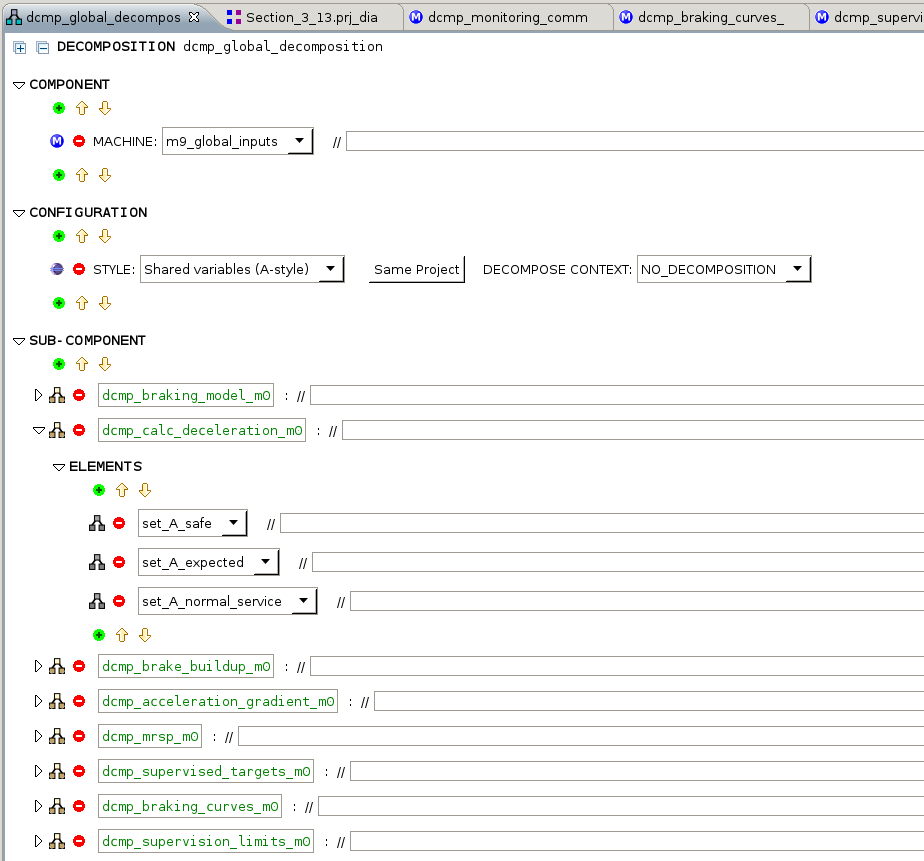
\includegraphics[width=.75\textwidth]{Decomp-Overview}
  \caption{Decomposition Configuration}
  \label{fig:decomp-overview}
\end{figure}

The overview of the decomposition in the Rodin tool using the decomposition
plug-in is shown in Fig.~\ref{fig:decomp-overview}. It lists the decomposed
machine, the decomposition style, the sub-components and the events in each
sub-machine (only shown for a single one).

In the following sections, the sub-components, their respective refinement and
the required context definitions will be explained.

\subsection{dcmp - Braking Model}
\label{sec:dcmp-braking-model}

The braking model has the following input variables: \bvar{a\_current},
\bvar{v\_current} and \bvar{loc\_current}. These variables are written by the
event \bevent{update\_train\_state}. The variables and this event are marked as
``DO NOT REFINE'', i.e., they are shared variables and an external event.

The output variables are \bvar{T\_brake\_service}, \bvar{T\_brake\_emergency},
\bvar{A\_brake\_normal\_service}, \bvar{A\_brake\_service} and
\bvar{A\_brake\_emergency}.

{\footnotesize
\begin{description}
\MACHINE{dcmp\_braking\_model\_m0}
\SEES{c6\_supervision\_limits}
\VARIABLES
        \begin{description}
                \ItemY{ A\_brake\_normal\_service }{Private variable}
                \ItemY{ A\_brake\_service }{Private variable}
                \ItemY{ a\_current }{Shared variable, DO NOT REFINE}
                \ItemY{ v\_current }{Shared variable, DO NOT REFINE}
                \ItemY{ T\_brake\_service }{Shared variable, DO NOT REFINE}
                \ItemY{ A\_brake\_emergency }{Private variable}
                \ItemY{ loc\_current }{Shared variable, DO NOT REFINE}
                \ItemY{ T\_brake\_emergency }{Shared variable, DO NOT REFINE}
        \end{description}
\EVENTS
        \EVT {update\_train\_state}\cmt{		\\\hspace*{4,2 cm}  External event, DO NOT REFINE }
                \begin{description}
                \AnyPrm
                        \begin{description}
                        \Item{l\_speed }
                        \Item{l\_accel }
                        \Item{l\_loc }
                        \end{description}
                \WhereGrd
                        \begin{description}
                        \nItem{ grd1 }{ l\_speed \in  t\_speed }
                        \nItem{ grd2 }{ l\_accel \in  t\_acceleration }
                        \nItem{ grd3 }{ l\_loc \in  t\_locations }
                        \end{description}
                \ThenAct
                        \begin{description}
                        \nItem{ act1 }{ v\_current :=  l\_speed }
                        \nItem{ act2 }{ a\_current :=  l\_accel }
                        \nItem{ act3 }{ loc\_current :=  l\_loc }
                        \end{description}
                \EndAct
                \end{description}
        \EVT {set\_A\_brake\_emergency}
                \begin{description}
                \AnyPrm
                        \begin{description}
                        \Item{l\_a\_brake }
                        \end{description}
                \WhereGrd
                        \begin{description}
                        \nItem{ grd1 }{ l\_a\_brake \in  t\_speed \tfun  t\_acceleration }
                        \end{description}
                \ThenAct
                        \begin{description}
                        \nItem{ act1 }{ A\_brake\_emergency :=  l\_a\_brake }
                        \end{description}
                \EndAct
                \end{description}
        \EVT {set\_A\_brake\_service}
                \begin{description}
                \AnyPrm
                        \begin{description}
                        \Item{l\_a\_brake }
                        \end{description}
                \WhereGrd
                        \begin{description}
                        \nItem{ grd1 }{ l\_a\_brake \in  t\_speed \tfun  t\_acceleration }
                        \end{description}
                \ThenAct
                        \begin{description}
                        \nItem{ act1 }{ A\_brake\_service :=  l\_a\_brake }
                        \end{description}
                \EndAct
                \end{description}
        \EVT {set\_A\_brake\_normal\_service}
                \begin{description}
                \AnyPrm
                        \begin{description}
                        \Item{l\_a\_brake }
                        \end{description}
                \WhereGrd
                        \begin{description}
                        \nItem{ grd1 }{ l\_a\_brake \in  t\_speed \tfun  t\_acceleration }
                        \end{description}
                \ThenAct
                        \begin{description}
                        \nItem{ act1 }{ A\_brake\_normal\_service :=  l\_a\_brake }
                        \end{description}
                \EndAct
                \end{description}
        \EVT {set\_T\_brake\_service}
                \begin{description}
                \AnyPrm
                        \begin{description}
                        \Item{l\_T\_brake }
                        \end{description}
                \WhereGrd
                        \begin{description}
                        \nItem{ grd1 }{ l\_T\_brake \in  t\_time }
                        \end{description}
                \ThenAct
                        \begin{description}
                        \nItem{ act1 }{ T\_brake\_service :=  l\_T\_brake }
                        \end{description}
                \EndAct
                \end{description}
        \EVT {set\_T\_brake\_emergency}
                \begin{description}
                \AnyPrm
                        \begin{description}
                        \Item{l\_T\_brake }
                        \end{description}
                \WhereGrd
                        \begin{description}
                        \nItem{ grd1 }{ l\_T\_brake \in  t\_time }
                        \end{description}
                \ThenAct
                        \begin{description}
                        \nItem{ act1 }{ T\_brake\_emergency :=  l\_T\_brake }
                        \end{description}
                \EndAct
                \end{description}
\END
\end{description}

}

\subsubsection{Context - Train Data 1 Brake}
\label{sec:context-train-data}

This context introduces the type \btype{t\_brake\_percentage} and a function
that takes the train speed, the brake percentage, the train length and the brake
position as arguments and returns a Boolean value indicating whether the
conversion model is applicable. It also introduces functions that calculate the
conversion model for the emergency and for the service brake, as well as the
conversion model for the brake buildup time of the service and emergency brake.

On the system level description of this Event-B model, these functions are not
implemented in more detail. Their specification and implementation details can
be found in §3.13.3 of the SRS.


{\footnotesize
\begin{description}
\CONTEXT{ctx\_train\_data\_1\_brake}
\EXTENDS{ctx\_train\_data}
\SETS
        \begin{description}
                \Item{ t\_brake\_position }
        \end{description}
\CONSTANTS
        \begin{description}
                \Item{ t\_brake\_percentage }
                \Item{ c\_brake\_percentage0 }
                \Item{ f\_conversion\_model\_applicable }
                \ItemY{ f\_conversion\_model\_A\_emergency }{}
                \Item{ f\_conversion\_model\_A\_service }
                \Item{ f\_conversion\_model\_T\_brake\_service }
                \Item{ f\_conversion\_model\_T\_brake\_emergency }
        \end{description}
\AXIOMS
        \begin{description}
                \nItem{ axm1 }{ t\_brake\_percentage \subseteq  t\_percentage }		\nItem{ axm2 }{ c\_brake\_percentage0 \in  t\_brake\_percentage }		\nItem{ axm3 }{ f\_conversion\_model\_applicable \in  t\_speed \cprod  t\_brake\_percentage \cprod  t\_length \cprod  t\_brake\_position \tfun  BOOL }\cmt{		\\\hspace*{1,4 cm}  cf. 3.13.3.2.1 }
                \nItem{ axm4 }{ f\_conversion\_model\_A\_emergency \in  t\_brake\_percentage \tfun  (t\_speed \tfun  t\_acceleration) }\cmt{		\\\hspace*{1,4 cm}  cf. 3.13.3.3 }
                \nItem{ axm5 }{ f\_conversion\_model\_A\_service \in  t\_brake\_percentage \tfun  (t\_speed \tfun  t\_acceleration) }		\nItem{ axm6 }{ f\_conversion\_model\_T\_brake\_service \in  t\_brake\_position \cprod  t\_length \cprod  t\_speed \tfun  t\_time }\cmt{		\\\hspace*{1,4 cm}  cf. 3.13.3.4 }
                \nItem{ axm7 }{ f\_conversion\_model\_T\_brake\_emergency \in  t\_brake\_position \cprod  t\_length \cprod  t\_speed \tfun  t\_time }	\end{description}
\END
\end{description}

}

\subsubsection{dcmp - Braking Model Conversion Model}
\label{sec:dcmp-braking-model-1}

In the first refinement of the sub-machine adds the variables
\bvar{brake\_percentage} of type brake percentage and
\bvar{brake\_percentage\_via\_train\_data} of Boolean type. These variables are
modified by the event \bevent{specify\_brake\_percentage} and
\bevent{remove\_brake\_percentage\_data}. The Boolean variable signals the
specification of the brake percentage via train data.

The value of the brake percentage is used in some events to compute concrete
values for the conversion model instead of using an event parameter. For example
in the event \bevent{calc\_A\_brake\_emergency\_conversion\_model}, the function
\bfunc{f\_conversion\_model\_A\_emergency} is used with the value
of\bvar{brake\_percentage} to compute the conversion model. This replaces the
event parameter \bparam{l\_a\_brake} by defining a \emph{witness} for it.

{\footnotesize
\begin{description}
\MACHINE{dcmp\_braking\_model\_m1\_conversion\_model}
\REFINES{dcmp\_braking\_model\_m0}
\SEES{c6\_supervision\_limits, ctx\_train\_data\_1\_brake}
\VARIABLES
        \begin{description}
                \ItemY{ brake\_percentage }{}
                \Item{ brake\_percentage\_via\_train\_data }
        \end{description}
\EVENTS
        \EVT {calc\_A\_brake\_emergency\_conversion\_model}
        \REF {set\_A\_brake\_emergency}
                \begin{description}
                \AnyPrm
                        \begin{description}
                        \Item{l\_brake\_position }
                        \end{description}
                \WhereGrd
                        \begin{description}
                        \nItem{ grd2 }{ brake\_percentage\_via\_train\_data = TRUE }
                        \nItem{ grd3 }{ f\_conversion\_model\_applicable (c\_train\_max\_speed \mapsto  brake\_percentage \mapsto  c\_train\_length \mapsto  l\_brake\_position) = TRUE }
                        \nItem{ grd4 }{ l\_brake\_position \in  t\_brake\_position }
                        \end{description}
                \Witnesses
                        \begin{description}
                        \nItemX{ l\_a\_brake }{ l\_a\_brake = f\_conversion\_model\_A\_emergency(brake\_percentage) }
                        \end{description}
                \ThenAct
                        \begin{description}
                        \nItem{ act1 }{ A\_brake\_emergency :=  f\_conversion\_model\_A\_emergency(brake\_percentage) }
                        \end{description}
                \EndAct
                \end{description}
        \EVT {calc\_A\_brake\_service\_conversion\_model}
        \REF {set\_A\_brake\_service}
                \begin{description}
                \AnyPrm
                        \begin{description}
                        \Item{l\_brake\_position }
                        \end{description}
                \WhereGrd
                        \begin{description}
                        \nItemY{ grd2 }{ brake\_percentage\_via\_train\_data = TRUE }{ }
                        \nItem{ grd3 }{ f\_conversion\_model\_applicable (c\_train\_max\_speed \mapsto  brake\_percentage \mapsto  c\_train\_length \mapsto  l\_brake\_position) = TRUE }
                        \nItem{ grd4 }{ l\_brake\_position \in  t\_brake\_position }
                        \end{description}
                \Witnesses
                        \begin{description}
                        \nItemX{ l\_a\_brake }{ l\_a\_brake = f\_conversion\_model\_A\_service(brake\_percentage) }
                        \end{description}
                \ThenAct
                        \begin{description}
                        \nItem{ act1 }{ A\_brake\_service :=  f\_conversion\_model\_A\_service(brake\_percentage) }
                        \end{description}
                \EndAct
                \end{description}
        \EVT {calc\_T\_brake\_service\_conversion\_model}
        \REF {set\_T\_brake\_service}
                \begin{description}
                \AnyPrm
                        \begin{description}
                        \ItemY{l\_brake\_position }{ }
                        \Item{l\_target\_speed }
                        \end{description}
                \WhereGrd
                        \begin{description}
                        \nItem{ grd2 }{ brake\_percentage\_via\_train\_data = TRUE }
                        \nItem{ grd3 }{ f\_conversion\_model\_applicable (c\_train\_max\_speed \mapsto  brake\_percentage \mapsto  c\_train\_length \mapsto  l\_brake\_position) = TRUE }
                        \nItem{ grd4 }{ l\_brake\_position \in  t\_brake\_position }
                        \nItem{ grd5 }{ l\_target\_speed \in  t\_speed }
                        \end{description}
                \Witnesses
                        \begin{description}
                        \nItemX{ l\_T\_brake }{ l\_T\_brake = f\_conversion\_model\_T\_brake\_service(l\_brake\_position \mapsto  c\_train\_length \mapsto  l\_target\_speed) }
                        \end{description}
                \ThenAct
                        \begin{description}
                        \nItem{ act1 }{ T\_brake\_service :=  f\_conversion\_model\_T\_brake\_service(l\_brake\_position \mapsto  c\_train\_length \mapsto  l\_target\_speed) }
                        \end{description}
                \EndAct
                \end{description}
        \REF {set\_T\_brake\_emergency}
                \begin{description}
                \AnyPrm
                        \begin{description}
                        \Item{l\_brake\_position }
                        \Item{l\_target\_speed }
                        \end{description}
                \WhereGrd
                        \begin{description}
                        \nItem{ grd1 }{ brake\_percentage\_via\_train\_data = TRUE }
                        \nItem{ grd2 }{ f\_conversion\_model\_applicable (c\_train\_max\_speed \mapsto  brake\_percentage \mapsto  c\_train\_length \mapsto  l\_brake\_position) = TRUE }
                        \nItem{ grd3 }{ l\_brake\_position \in  t\_brake\_position }
                        \nItem{ grd4 }{ l\_target\_speed \in  t\_speed }
                        \end{description}
                \Witnesses
                        \begin{description}
                        \nItemX{ l\_T\_brake }{ l\_T\_brake = f\_conversion\_model\_T\_brake\_emergency(l\_brake\_position \mapsto  c\_train\_length \mapsto  l\_target\_speed) }
                        \end{description}
                \ThenAct
                        \begin{description}
                        \nItem{ act1 }{ T\_brake\_emergency :=  f\_conversion\_model\_T\_brake\_emergency(l\_brake\_position \mapsto  c\_train\_length \mapsto  l\_target\_speed) }
                        \end{description}
                \EndAct
                \end{description}
        \EVT {specifiy\_brake\_percentage}
                \begin{description}
                \AnyPrm
                        \begin{description}
                        \ItemY{l\_brake }{ }
                        \end{description}
                \WhereGrd
                        \begin{description}
                        \nItem{ grd1 }{ l\_brake \in  t\_brake\_percentage }
                        \nItem{ grd2 }{ brake\_percentage\_via\_train\_data = FALSE }
                        \end{description}
                \ThenAct
                        \begin{description}
                        \nItem{ act1 }{ brake\_percentage :=  l\_brake }
                        \nItem{ act2 }{ brake\_percentage\_via\_train\_data :=  TRUE }
                        \end{description}
                \EndAct
                \end{description}
        \EVT {remove\_brake\_percentage\_data}
                \begin{description}
                \WhenGrd
                        \begin{description}
                        \nItem{ grd1 }{ brake\_percentage\_via\_train\_data = TRUE }
                        \end{description}
                \ThenAct
                        \begin{description}
                        \nItem{ act1 }{ brake\_percentage :=  c\_brake\_percentage0 }
                        \nItem{ act2 }{ brake\_percentage\_via\_train\_data :=  FALSE }
                        \end{description}
                \EndAct
                \end{description}
\END
\end{description}

}

\subsubsection{Context - Train Data 2 Direct Calculation}
\label{sec:context-train-data-1}

The next context introduces the type representing the combination of the
different brake types of the train. It also defines functions that calculate the
braking models for different brake combinations for the service brake and the
emergency brake, as well as functions to calculate the brake buildup time for
the service and emergency brake with the brake combination as argument. It also
defines a function that calculates the normal brake function dependent on the
brake position and the acceleration constants \bconst{c\_SB01} and
\bconst{c\_SB02} (cf.~§3.13.2.2.3.1.10).

{\footnotesize
\begin{description}
\CONTEXT{ctx\_train\_data\_2\_dircect\_calc}
\EXTENDS{ctx\_train\_data\_1\_brake}
\SETS
        \begin{description}
                \ItemY{ t\_brake\_combination }{cf. 3.13.2.2.3.1.7, i.e., combination of regenerative, eddy current and magnetic brake }
        \end{description}
\CONSTANTS
        \begin{description}
                \ItemY{ c\_v\_zero }{target speed zero}
                \Item{ f\_calc\_A\_brake\_service\_direct }
                \Item{ f\_calc\_A\_brake\_emergency\_direct }
                \ItemY{ f\_calc\_A\_brake\_normal\_direct }{cf. 3.13.2.2.3.1.9}
                \Item{ c\_SB01 }
                \Item{ c\_SB02 }
                \Item{ f\_calc\_T\_brake\_service }
                \Item{ f\_calc\_T\_brake\_emergency }
        \end{description}
\AXIOMS
        \begin{description}
                \nItem{ axm1 }{ c\_v\_zero \in  t\_speed }		\nItem{ axm2 }{ f\_calc\_A\_brake\_service\_direct \in  t\_brake\_combination \tfun  (t\_speed \tfun  t\_acceleration) }		\nItem{ axm3 }{ f\_calc\_A\_brake\_emergency\_direct \in  t\_brake\_combination \tfun  (t\_speed \tfun  t\_acceleration) }		\nItem{ axm4 }{ f\_calc\_A\_brake\_normal\_direct \in  t\_brake\_position \cprod  t\_acceleration \cprod  t\_acceleration		\\\hspace*{7,6 cm}  \tfun  (t\_speed \tfun  t\_acceleration) }\cmt{		\\\hspace*{1,4 cm}  cf. 3.13.2.2.3.1.10		\\\hspace*{1,2 cm}  the accelerations are the c$\_$SB01 and c$\_$SB02 constants }
                \nItem{ axm5 }{ c\_SB01 \in  t\_acceleration }		\nItem{ axm6 }{ c\_SB02 \in  t\_acceleration }		\nItem{ axm7 }{ f\_calc\_T\_brake\_service \in  t\_brake\_combination \tfun  t\_time }		\nItem{ axm8 }{ f\_calc\_T\_brake\_emergency \in  t\_brake\_combination \tfun  t\_time }	\end{description}
\END
\end{description}

}

\subsubsection{dcmp - Braking Model Direct Calculation}
\label{sec:dcmp-braking-model-2}

This machine refinement uses the brake combinations and the corresponding
functions from the context to produce more concrete events. For events that
compute a function mapping speed to acceleration, the functions of the context
and the constants for SB01 and SB02 are used to eliminate the event parameters
by providing witnesses for them.

{\footnotesize
\begin{description}
\MACHINE{dcmp\_braking\_model\_m2\_direct\_calc}
\REFINES{dcmp\_braking\_model\_m1\_conversion\_model}
\SEES{c6\_supervision\_limits, ctx\_train\_data\_2\_dircect\_calc}
\EVENTS
        \EVT {calc\_A\_brake\_emergency\_direct}
        \REF {set\_A\_brake\_emergency}
                \begin{description}
                \AnyPrm
                        \begin{description}
                        \Item{l\_brake\_combination }
                        \end{description}
                \WhereGrd
                        \begin{description}
                        \nItem{ grd1 }{ l\_brake\_combination \in  t\_brake\_combination }
                        \end{description}
                \Witnesses
                        \begin{description}
                        \nItemX{ l\_a\_brake }{ l\_a\_brake = f\_calc\_A\_brake\_emergency\_direct(l\_brake\_combination) }
                        \end{description}
                \ThenAct
                        \begin{description}
                        \nItem{ act1 }{ A\_brake\_emergency :=  f\_calc\_A\_brake\_emergency\_direct(l\_brake\_combination) }
                        \end{description}
                \EndAct
                \end{description}
        \EVT {calc\_A\_brake\_service\_direct}
        \REF {set\_A\_brake\_service}
                \begin{description}
                \AnyPrm
                        \begin{description}
                        \Item{l\_brake\_combination }
                        \end{description}
                \WhereGrd
                        \begin{description}
                        \nItemY{ grd2 }{ l\_brake\_combination \in  t\_brake\_combination }{ }
                        \end{description}
                \Witnesses
                        \begin{description}
                        \nItemX{ l\_a\_brake }{ l\_a\_brake = f\_calc\_A\_brake\_service\_direct(l\_brake\_combination) }
                        \end{description}
                \ThenAct
                        \begin{description}
                        \nItem{ act1 }{ A\_brake\_service :=  f\_calc\_A\_brake\_service\_direct(l\_brake\_combination) }
                        \end{description}
                \EndAct
                \end{description}
        \EVT {set\_A\_brake\_normal\_service}
        \REF {set\_A\_brake\_normal\_service}
                \begin{description}
                \AnyPrm
                        \begin{description}
                        \Item{l\_brake\_position }
                        \end{description}
                \WhereGrd
                        \begin{description}
                        \nItem{ grd1 }{ l\_brake\_position \in  t\_brake\_position }
                        \end{description}
                \Witnesses
                        \begin{description}
                        \nItemX{ l\_a\_brake }{ l\_a\_brake = f\_calc\_A\_brake\_normal\_direct(l\_brake\_position \mapsto  c\_SB01 \mapsto  c\_SB02) }
                        \end{description}
                \ThenAct
                        \begin{description}
                        \nItem{ act1 }{ A\_brake\_normal\_service :=  f\_calc\_A\_brake\_normal\_direct(l\_brake\_position \mapsto  c\_SB01 \mapsto  c\_SB02) }
                        \end{description}
                \EndAct
                \end{description}
        \EVT {set\_T\_brake\_service}\cmt{ }
        \REF {set\_T\_brake\_service}
                \begin{description}
                \AnyPrm
                        \begin{description}
                        \Item{l\_brake\_combination }
                        \end{description}
                \WhereGrd
                        \begin{description}
                        \nItem{ grd1 }{ l\_brake\_combination \in  t\_brake\_combination }
                        \end{description}
                \Witnesses
                        \begin{description}
                        \nItemX{ l\_T\_brake }{ l\_T\_brake = f\_calc\_T\_brake\_service(l\_brake\_combination) }
                        \end{description}
                \ThenAct
                        \begin{description}
                        \nItemY{ act1 }{ T\_brake\_service :=  f\_calc\_T\_brake\_service(l\_brake\_combination) }{  }
                        \end{description}
                \EndAct
                \end{description}
        \EVT {set\_T\_brake\_emergency}
        \REF {set\_T\_brake\_emergency}
                \begin{description}
                \AnyPrm
                        \begin{description}
                        \Item{l\_brake\_combination }
                        \end{description}
                \WhereGrd
                        \begin{description}
                        \nItem{ grd1 }{ l\_brake\_combination \in  t\_brake\_combination }
                        \end{description}
                \Witnesses
                        \begin{description}
                        \nItemX{ l\_T\_brake }{ l\_T\_brake = f\_calc\_T\_brake\_emergency(l\_brake\_combination) }
                        \end{description}
                \ThenAct
                        \begin{description}
                        \nItem{ act1 }{ T\_brake\_emergency :=  f\_calc\_T\_brake\_emergency(l\_brake\_combination) }
                        \end{description}
                \EndAct
                \end{description}
\END
\end{description}

}

\subsection{dcmp - Calc Deceleration}
\label{sec:dcmp-calc-decel}

The deceleration calculation model has the following input variables:
\bvar{a\_current}, \bvar{v\_current} and \bvar{loc\_current}. The output
variables it calculates are \bvar{A\_normal\_service}, \bvar{A\_expected} and
\bvar{A\_safe} which each map train speed and distance to an acceleration.

{\footnotesize
\begin{description}
\MACHINE{dcmp\_calc\_deceleration\_m0}
\SEES{c6\_supervision\_limits}
\EVENTS
        \EVT {set\_A\_safe}
                \begin{description}
                \AnyPrm
                        \begin{description}
                        \Item{l\_a\_decel }
                        \end{description}
                \WhereGrd
                        \begin{description}
                        \nItem{ grd1 }{ l\_a\_decel \in  t\_speed \cprod  t\_distance \tfun  t\_acceleration }
                        \end{description}
                \ThenAct
                        \begin{description}
                        \nItem{ act1 }{ A\_safe :=  l\_a\_decel }
                        \end{description}
                \EndAct
                \end{description}
        \EVT {set\_A\_expected}
                \begin{description}
                \AnyPrm
                        \begin{description}
                        \Item{l\_a\_decel }
                        \end{description}
                \WhereGrd
                        \begin{description}
                        \nItem{ grd1 }{ l\_a\_decel \in  t\_speed \cprod  t\_distance \tfun  t\_acceleration }
                        \end{description}
                \ThenAct
                        \begin{description}
                        \nItem{ act1 }{ A\_expected :=  l\_a\_decel }
                        \end{description}
                \EndAct
                \end{description}
        \EVT {set\_A\_normal\_service}
                \begin{description}
                \AnyPrm
                        \begin{description}
                        \Item{l\_a\_decel }
                        \end{description}
                \WhereGrd
                        \begin{description}
                        \nItem{ grd1 }{ l\_a\_decel \in  t\_speed \cprod  t\_distance \tfun  t\_acceleration }
                        \end{description}
                \ThenAct
                        \begin{description}
                        \nItem{ act1 }{ A\_normal\_service :=  l\_a\_decel }
                        \end{description}
                \EndAct
                \end{description}
\END
\end{description}

}

\subsection{dcmp - Brake Buildup}
\label{sec:dcmp-brake-buildup}

The brake buildup time calculation has the following input variables:
\bvar{a\_current}, \bvar{v\_current} and \bvar{loc\_current}. The output
variables are \bvar{T\_be}, \bvar{T\_se}, \bvar{T\_brake\_service} and
\bvar{T\_brake\_emergency}.

{\footnotesize
\begin{description}
\MACHINE{dcmp\_brake\_buildup\_m0}
\SEES{c6\_supervision\_limits}
\VARIABLES
        \begin{description}
                \ItemY{ T\_be }{Shared variable, DO NOT REFINE}
                \ItemY{ T\_bs }{Shared variable, DO NOT REFINE}
                \ItemY{ a\_current }{Shared variable, DO NOT REFINE}
                \ItemY{ v\_current }{Shared variable, DO NOT REFINE}
                \ItemY{ T\_brake\_service }{Shared variable, DO NOT REFINE}
                \ItemY{ loc\_current }{Shared variable, DO NOT REFINE}
                \ItemY{ T\_brake\_emergency }{Shared variable, DO NOT REFINE}
        \end{description}
\INVARIANTS
        \begin{description}
                \nItem{ typing\_T\_be }{ T\_be \in  t\_time }
                \nItem{ typing\_T\_bs }{ T\_bs \in  t\_time }
                \nItem{ typing\_a\_current }{ a\_current \in  t\_acceleration }
                \nItem{ typing\_v\_current }{ v\_current \in  t\_speed }
                \nItem{ typing\_T\_brake\_service }{ T\_brake\_service \in  t\_time }
                \nItem{ typing\_loc\_current }{ loc\_current \in  t\_locations }
                \nItem{ typing\_T\_brake\_emergency }{ T\_brake\_emergency \in  t\_time }
        \end{description}
\EVENTS
        \INITIALISATION
                \begin{description}
                \BeginAct
                        \begin{description}
                        \nItem{ act1 }{ v\_current :=  c\_v0 }
                        \nItem{ act2 }{ a\_current :=  c\_a0 }
                        \nItem{ act3 }{ loc\_current :=  c\_l0 }
                        \nItem{ act9 }{ T\_brake\_service :=  c\_T\_brake0 }
                        \nItem{ act10 }{ T\_brake\_emergency :=  c\_T\_brake0 }
                        \nItem{ act14 }{ T\_be :=  c\_T\_brake0 }
                        \nItem{ act15 }{ T\_bs :=  c\_T\_brake0 }
                        \end{description}
                \EndAct
                \end{description}
        \EVT {update\_train\_state}\cmt{		\\\hspace*{4,2 cm}  External event, DO NOT REFINE }
                \begin{description}
                \AnyPrm
                        \begin{description}
                        \Item{l\_speed }
                        \Item{l\_accel }
                        \Item{l\_loc }
                        \end{description}
                \WhereGrd
                        \begin{description}
                        \nItem{ grd1 }{ l\_speed \in  t\_speed }
                        \nItem{ grd2 }{ l\_accel \in  t\_acceleration }
                        \nItem{ grd3 }{ l\_loc \in  t\_locations }
                        \end{description}
                \ThenAct
                        \begin{description}
                        \nItem{ act1 }{ v\_current :=  l\_speed }
                        \nItem{ act2 }{ a\_current :=  l\_accel }
                        \nItem{ act3 }{ loc\_current :=  l\_loc }
                        \end{description}
                \EndAct
                \end{description}
        \EVT {set\_T\_brake\_service}\cmt{		\\\hspace*{4,4 cm}  External event, DO NOT REFINE }
                \begin{description}
                \AnyPrm
                        \begin{description}
                        \Item{l\_T\_brake }
                        \end{description}
                \WhereGrd
                        \begin{description}
                        \nItem{ grd1 }{ l\_T\_brake \in  t\_time }
                        \end{description}
                \ThenAct
                        \begin{description}
                        \nItem{ act1 }{ T\_brake\_service :=  l\_T\_brake }
                        \end{description}
                \EndAct
                \end{description}
        \EVT {set\_T\_brake\_emergency}\cmt{		\\\hspace*{4,8 cm}  External event, DO NOT REFINE }
                \begin{description}
                \AnyPrm
                        \begin{description}
                        \Item{l\_T\_brake }
                        \end{description}
                \WhereGrd
                        \begin{description}
                        \nItem{ grd1 }{ l\_T\_brake \in  t\_time }
                        \end{description}
                \ThenAct
                        \begin{description}
                        \nItem{ act1 }{ T\_brake\_emergency :=  l\_T\_brake }
                        \end{description}
                \EndAct
                \end{description}
        \EVT {set\_T\_be}
                \begin{description}
                \AnyPrm
                        \begin{description}
                        \Item{l\_t\_be }
                        \end{description}
                \WhereGrd
                        \begin{description}
                        \nItem{ grd1 }{ l\_t\_be \in  t\_time }
                        \end{description}
                \ThenAct
                        \begin{description}
                        \nItem{ act1 }{ T\_be :=  l\_t\_be }
                        \end{description}
                \EndAct
                \end{description}
        \EVT {set\_T\_bs}
                \begin{description}
                \AnyPrm
                        \begin{description}
                        \Item{l\_t\_bs }
                        \end{description}
                \WhereGrd
                        \begin{description}
                        \nItem{ grd1 }{ l\_t\_bs \in  t\_time }
                        \end{description}
                \ThenAct
                        \begin{description}
                        \nItem{ act1 }{ T\_bs :=  l\_t\_bs }
                        \end{description}
                \EndAct
                \end{description}
\END
\end{description}

}

\subsubsection{Context - Brake Buildup Functions}
\label{sec:cont-brake-build}

This context defines 4 functions that calculate the brake buildup time for the
service and emergency brake. For each there are two functions, one for the
conversion model and one without conversion model. The service break is not
safety-critical, therefore it does not take a correction factor into account
(cf.~§3.13.6.3.1.1).

\begin{description}
\CONTEXT{ctx\_functions\_1\_calc\_T\_brake}
\EXTENDS{ctx\_functions\_0}
\CONSTANTS
        \begin{description}
                \Item{ f\_T\_brake\_service\_conversion }
                \Item{ f\_T\_brake\_service }
                \ItemY{ f\_T\_brake\_emergency\_conversion }{}
                \Item{ f\_T\_brake\_emergency }
        \end{description}
\AXIOMS
        \begin{description}
                \nItem{ axm1 }{ f\_T\_brake\_service\_conversion \in  t\_time \cprod  t\_brake\_combination \tfun  t\_time }\cmt{ }
                \nItem{ axm2 }{ f\_T\_brake\_service \in  t\_time \cprod  t\_brake\_combination \tfun  t\_time }		\nItem{ axm3 }{ f\_T\_brake\_emergency\_conversion \in  t\_time \cprod  t\_correction\_factor \tfun  t\_time }		\nItem{ axm4 }{ f\_T\_brake\_emergency \in  t\_time \cprod  t\_brake\_combination \tfun  t\_time }	\end{description}
\END
\end{description}



\subsubsection{dcmp - Brake Buildup Calculation}
\label{sec:dcmp-brake-buildup-1}

This refinement applies the calculation functions defined in the context to the
calculation events. It adds the notions of train data to the machine which
controls whether the conversion model is used for the brake buildup time
calculation. This is represented by two variables each, a Boolean variable that
signals whether a concrete train data has been supplied and a variable of type
\btype{t\_time} representing the supplied value.

{\footnotesize
\begin{description}
\MACHINE{dcmp\_brake\_buildup\_m2\_calculation}
\REFINES{dcmp\_brake\_buildup\_m0}
\SEES{c6\_supervision\_limits, ctx\_functions\_1\_calc\_T\_brake}
\VARIABLES
        \begin{description}
                \ItemY{ T\_be }{Shared variable, DO NOT REFINE}
                \ItemY{ T\_bs }{Shared variable, DO NOT REFINE}
                \ItemY{ a\_current }{Shared variable, DO NOT REFINE}
                \ItemY{ v\_current }{Shared variable, DO NOT REFINE}
                \ItemY{ T\_brake\_service }{Shared variable, DO NOT REFINE}
                \ItemY{ loc\_current }{Shared variable, DO NOT REFINE}
                \ItemY{ T\_brake\_emergency }{Shared variable, DO NOT REFINE}
                \Item{ T\_brake\_service\_data }
                \ItemY{ T\_brake\_service\_via\_train\_data }{}
                \Item{ T\_brake\_emergency\_data }
                \Item{ T\_brake\_emergency\_via\_train\_data }
        \end{description}
\INVARIANTS
        \begin{description}
                \nItem{ inv1 }{ T\_brake\_service\_data \in  t\_time }
                \nItem{ inv2 }{ T\_brake\_service\_via\_train\_data \in  BOOL }
                \nItem{ inv3 }{ T\_brake\_emergency\_data \in  t\_time }
                \nItem{ inv4 }{ T\_brake\_emergency\_via\_train\_data \in  BOOL }
        \end{description}
\EVENTS
        \INITIALISATION
                \\\textit{extended}
                \begin{description}
                \BeginAct
                        \begin{description}
                        \nItemX{ act1 }{ v\_current :=  c\_v0 }
                        \nItemX{ act2 }{ a\_current :=  c\_a0 }
                        \nItemX{ act3 }{ loc\_current :=  c\_l0 }
                        \nItemX{ act9 }{ T\_brake\_service :=  c\_T\_brake0 }
                        \nItemX{ act10 }{ T\_brake\_emergency :=  c\_T\_brake0 }
                        \nItemX{ act14 }{ T\_be :=  c\_T\_brake0 }
                        \nItemX{ act15 }{ T\_bs :=  c\_T\_brake0 }
                        \nItem{ act16 }{ T\_brake\_service\_data :=  c\_T\_brake0 }
                        \nItem{ act17 }{ T\_brake\_service\_via\_train\_data :=  FALSE }
                        \nItem{ act18 }{ T\_brake\_emergency\_data :=  c\_T\_brake0 }
                        \nItem{ act19 }{ T\_brake\_emergency\_via\_train\_data :=  FALSE }
                        \end{description}
                \EndAct
                \end{description}
        \EVT {update\_train\_state}\cmt{		\\\hspace*{4,2 cm}  External event, DO NOT REFINE }
        \EXTD {update\_train\_state}
                \begin{description}
                \AnyPrm
                        \begin{description}
                        \ItemX{l\_speed }
                        \ItemX{l\_accel }
                        \ItemX{l\_loc }
                        \end{description}
                \WhereGrd
                        \begin{description}
                        \nItemX{ grd1 }{ l\_speed \in  t\_speed }
                        \nItemX{ grd2 }{ l\_accel \in  t\_acceleration }
                        \nItemX{ grd3 }{ l\_loc \in  t\_locations }
                        \end{description}
                \ThenAct
                        \begin{description}
                        \nItemX{ act1 }{ v\_current :=  l\_speed }
                        \nItemX{ act2 }{ a\_current :=  l\_accel }
                        \nItemX{ act3 }{ loc\_current :=  l\_loc }
                        \end{description}
                \EndAct
                \end{description}
        \EVT {set\_T\_brake\_service}\cmt{		\\\hspace*{4,4 cm}  External event, DO NOT REFINE }
        \EXTD {set\_T\_brake\_service}
                \begin{description}
                \AnyPrm
                        \begin{description}
                        \ItemX{l\_T\_brake }
                        \end{description}
                \WhereGrd
                        \begin{description}
                        \nItemX{ grd1 }{ l\_T\_brake \in  t\_time }
                        \end{description}
                \ThenAct
                        \begin{description}
                        \nItemX{ act1 }{ T\_brake\_service :=  l\_T\_brake }
                        \end{description}
                \EndAct
                \end{description}
        \EVT {set\_T\_brake\_emergency}\cmt{		\\\hspace*{4,8 cm}  External event, DO NOT REFINE }
        \EXTD {set\_T\_brake\_emergency}
                \begin{description}
                \AnyPrm
                        \begin{description}
                        \ItemX{l\_T\_brake }
                        \end{description}
                \WhereGrd
                        \begin{description}
                        \nItemX{ grd1 }{ l\_T\_brake \in  t\_time }
                        \end{description}
                \ThenAct
                        \begin{description}
                        \nItemX{ act1 }{ T\_brake\_emergency :=  l\_T\_brake }
                        \end{description}
                \EndAct
                \end{description}
        \EVT {set\_T\_be}
        \REF {set\_T\_be}
                \begin{description}
                \AnyPrm
                        \begin{description}
                        \Item{l\_brake\_combination }
                        \end{description}
                \WhereGrd
                        \begin{description}
                        \nItem{ grd1 }{ T\_brake\_emergency\_via\_train\_data = TRUE }
                        \nItem{ grd2 }{ l\_brake\_combination \in  t\_brake\_combination }
                        \end{description}
                \Witnesses
                        \begin{description}
                        \nItemX{ l\_t\_be }{ l\_t\_be = f\_T\_brake\_emergency(T\_brake\_emergency \mapsto  l\_brake\_combination) }
                        \end{description}
                \ThenAct
                        \begin{description}
                        \nItemY{ act1 }{ T\_be :=  f\_T\_brake\_emergency(T\_brake\_emergency \mapsto  l\_brake\_combination) }{  }
                        \end{description}
                \EndAct
                \end{description}
        \EVT {calc\_T\_be\_conversion\_model}
        \REF {set\_T\_brake\_emergency}
                \begin{description}
                \WhenGrd
                        \begin{description}
                        \nItem{ grd1 }{ T\_brake\_emergency\_via\_train\_data = FALSE }
                        \end{description}
                \Witnesses
                        \begin{description}
                        \nItemX{ l\_T\_brake }{ l\_T\_brake = f\_T\_brake\_emergency\_conversion(T\_brake\_service \mapsto  c\_Kt\_int) }{ }
                        \end{description}
                \ThenAct
                        \begin{description}
                        \nItem{ act1 }{ T\_brake\_emergency :=  f\_T\_brake\_emergency\_conversion(T\_brake\_service \mapsto  c\_Kt\_int) }
                        \end{description}
                \EndAct
                \end{description}
        \EVT {set\_T\_bs}
        \REF {set\_T\_bs}
                \begin{description}
                \AnyPrm
                        \begin{description}
                        \Item{l\_brake\_combination }
                        \end{description}
                \WhereGrd
                        \begin{description}
                        \nItem{ grd1 }{ T\_brake\_service\_via\_train\_data = TRUE }
                        \nItem{ grd2 }{ l\_brake\_combination \in  t\_brake\_combination }
                        \end{description}
                \Witnesses
                        \begin{description}
                        \nItemX{ l\_t\_bs }{ l\_t\_bs = f\_T\_brake\_service(T\_brake\_service\_data \mapsto  l\_brake\_combination) }
                        \end{description}
                \ThenAct
                        \begin{description}
                        \nItem{ act1 }{ T\_bs :=  f\_T\_brake\_service(T\_brake\_service\_data \mapsto  l\_brake\_combination) }
                        \end{description}
                \EndAct
                \end{description}
        \EVT {calc\_T\_bs\_conversion\_model}
        \REF {set\_T\_bs}
                \begin{description}
                \AnyPrm
                        \begin{description}
                        \Item{l\_brake\_combination }
                        \end{description}
                \WhereGrd
                        \begin{description}
                        \nItem{ grd1 }{ T\_brake\_service\_via\_train\_data = FALSE }
                        \nItem{ grd2 }{ l\_brake\_combination \in  t\_brake\_combination }
                        \end{description}
                \Witnesses
                        \begin{description}
                        \nItemX{ l\_t\_bs }{ l\_t\_bs = f\_T\_brake\_emergency(T\_brake\_service \mapsto  l\_brake\_combination) }
                        \end{description}
                \ThenAct
                        \begin{description}
                        \nItem{ act1 }{ T\_bs :=  f\_T\_brake\_emergency(T\_brake\_service \mapsto  l\_brake\_combination) }
                        \end{description}
                \EndAct
                \end{description}
        \EVT {specify\_T\_brake\_service\_train\_data}
                \begin{description}
                \AnyPrm
                        \begin{description}
                        \Item{l\_T\_brake }
                        \end{description}
                \WhereGrd
                        \begin{description}
                        \nItem{ grd1 }{ l\_T\_brake \in  t\_time }
                        \nItemY{ grd2 }{ T\_brake\_service\_via\_train\_data = FALSE }{ }
                        \end{description}
                \ThenAct
                        \begin{description}
                        \nItem{ act1 }{ T\_brake\_service\_data :=  l\_T\_brake }
                        \nItem{ act2 }{ T\_brake\_service\_via\_train\_data :=  TRUE }
                        \end{description}
                \EndAct
                \end{description}
        \EVT {remove\_T\_brake\_service\_data}
                \begin{description}
                \WhenGrd
                        \begin{description}
                        \nItem{ grd1 }{ T\_brake\_service\_via\_train\_data = TRUE }
                        \end{description}
                \ThenAct
                        \begin{description}
                        \nItem{ act1 }{ T\_brake\_service\_via\_train\_data :=  FALSE }
                        \end{description}
                \EndAct
                \end{description}
        \EVT {specify\_T\_brake\_emergency\_train\_data}
                \begin{description}
                \AnyPrm
                        \begin{description}
                        \Item{l\_T\_brake }
                        \end{description}
                \WhereGrd
                        \begin{description}
                        \nItem{ grd1 }{ l\_T\_brake \in  t\_time }
                        \nItem{ grd2 }{ T\_brake\_emergency\_via\_train\_data = FALSE }
                        \end{description}
                \ThenAct
                        \begin{description}
                        \nItem{ act1 }{ T\_brake\_emergency\_data :=  l\_T\_brake }
                        \nItem{ act2 }{ T\_brake\_emergency\_via\_train\_data :=  TRUE }
                        \end{description}
                \EndAct
                \end{description}
        \EVT {remove\_T\_brake\_emergency\_data}
                \begin{description}
                \WhenGrd
                        \begin{description}
                        \nItem{ grd1 }{ T\_brake\_emergency\_via\_train\_data = TRUE }
                        \end{description}
                \ThenAct
                        \begin{description}
                        \nItem{ act1 }{ T\_brake\_emergency\_via\_train\_data :=  FALSE }
                        \end{description}
                \EndAct
                \end{description}
\END
\end{description}

}

\subsection{dcmp - Acceleration Gradient}
\label{sec:dcmp-accel-grad}

The calculation of the acceleration gradient has the current train state as
input values (i.e., speed, location and acceleration). Its output value is the
acceleration due to gradient, represented by the variable \bvar{A\_gradient}.

{\footnotesize
\begin{description}
\MACHINE{dcmp\_acceleration\_gradient\_m0}
\SEES{c6\_supervision\_limits}
\VARIABLES
        \begin{description}
                \ItemY{ a\_current }{Shared variable, DO NOT REFINE}
                \ItemY{ v\_current }{Shared variable, DO NOT REFINE}
                \ItemY{ loc\_current }{Shared variable, DO NOT REFINE}
                \ItemY{ A\_gradient }{Private variable}
        \end{description}
\INVARIANTS
        \begin{description}
                \nItem{ typing\_a\_current }{ a\_current \in  t\_acceleration }
                \nItem{ typing\_v\_current }{ v\_current \in  t\_speed }
                \nItem{ typing\_loc\_current }{ loc\_current \in  t\_locations }
                \nItem{ typing\_A\_gradient }{ A\_gradient \in  t\_acceleration }
                \nItem{ m4\_accel\_decel\_gradient\_inv1 }{ A\_gradient \in  t\_acceleration }
        \end{description}
\EVENTS
        \INITIALISATION
                \begin{description}
                \BeginAct
                        \begin{description}
                        \nItem{ act1 }{ v\_current :=  c\_v0 }
                        \nItem{ act2 }{ a\_current :=  c\_a0 }
                        \nItem{ act3 }{ loc\_current :=  c\_l0 }
                        \nItem{ act16 }{ A\_gradient :=  c\_a0 }
                        \end{description}
                \EndAct
                \end{description}
        \EVT {update\_train\_state}\cmt{		\\\hspace*{4,2 cm}  External event, DO NOT REFINE }
                \begin{description}
                \AnyPrm
                        \begin{description}
                        \Item{l\_speed }
                        \Item{l\_accel }
                        \Item{l\_loc }
                        \end{description}
                \WhereGrd
                        \begin{description}
                        \nItem{ grd1 }{ l\_speed \in  t\_speed }
                        \nItem{ grd2 }{ l\_accel \in  t\_acceleration }
                        \nItem{ grd3 }{ l\_loc \in  t\_locations }
                        \end{description}
                \ThenAct
                        \begin{description}
                        \nItem{ act1 }{ v\_current :=  l\_speed }
                        \nItem{ act2 }{ a\_current :=  l\_accel }
                        \nItem{ act3 }{ loc\_current :=  l\_loc }
                        \end{description}
                \EndAct
                \end{description}
        \EVT {set\_A\_gradient}
                \begin{description}
                \AnyPrm
                        \begin{description}
                        \ItemY{l\_a\_gradient }{ }
                        \end{description}
                \WhereGrd
                        \begin{description}
                        \nItemY{ grd1 }{ l\_a\_gradient \in  t\_acceleration }{ }
                        \end{description}
                \ThenAct
                        \begin{description}
                        \nItem{ act1 }{ A\_gradient :=  l\_a\_gradient }
                        \end{description}
                \EndAct
                \end{description}
\END
\end{description}

}


\subsubsection{Context - MRSP and Gradients}
\label{sec:cont-mrsp-grad}

This context introduces functions to calculate an acceleration due to gradient
(cf.~3.13.4) and to calculate the current most restrictive speed profile from
the set of applicable speed profiles for a location.

\begin{description}
\CONTEXT{ctx\_functions\_0}
\EXTENDS{ctx\_type\_gradients}
\CONSTANTS
        \begin{description}
                \Item{ f\_accel\_due\_gradient }
                \Item{ f\_grad\_uphill }
                \Item{ f\_compensate\_gradient\_profile }
                \Item{ f\_mrsp }
        \end{description}
\AXIOMS
        \begin{description}
                \nItem{ axm1 }{ f\_accel\_due\_gradient \in             \\\hspace*{1,2 cm}  t\_locations \cprod  t\_locations \cprod  t\_gradients \cprod  t\_mass\_percentage \cprod  t\_speed\_profiles \tfun  t\_acceleration }\cmt{		\\\hspace*{1,4 cm}  (loc, SvL, compensated$\_$grad, mass, speed$\_$profile)		\\\hspace*{1,2 cm}  calculates acceleration due to gradient according to 3.13.4 }
                \nItem{ axm2 }{ f\_grad\_uphill \in  t\_gradients \tfun  BOOL }\cmt{		\\\hspace*{1,4 cm}  indicates whether gradient is uphil or downhill }
                \nItem{ axm3 }{ f\_compensate\_gradient\_profile \in  t\_locations \cprod  t\_locations \cprod  t\_gradient\_profiles \tfun  t\_gradients }\cmt{		\\\hspace*{1,4 cm}  (loc, SvL, profile) compensates for gradient profile (cf. 3.13.4.2.1) }
                \nItem{ axm4 }{ f\_mrsp \in  t\_speed\_profiles \cprod  t\_speed\_profiles \cprod  t\_speed\_profiles \cprod  t\_speed\_profiles		\\\hspace*{2,6 cm}  \cprod  t\_speed\_profiles \cprod  t\_speed\_profiles \cprod  t\_speed\_profiles \cprod  t\_speed\_profiles		\\\hspace*{2,6 cm}  \cprod  t\_train\_modes \cprod  t\_speed \cprod  t\_length \tfun  t\_speed\_profiles }\cmt{		\\\hspace*{1,4 cm}  function which calculates the most restrictive speed profile		\\\hspace*{1,2 cm}  (MRSP) from the following inputs:		\\\hspace*{1,2 cm}  SSP, Axle Load SP, TSR, signalling related, mode related, LX speed,		\\\hspace*{1,2 cm}  override function related, SR to ensure permitted brake distance,		\\\hspace*{1,2 cm}  train mode, max train speed, train length }
        \end{description}
\END
\end{description}



\subsubsection{dcmp - Rotating Mass}
\label{sec:dcmp-rotating-mass}

This machine introduces the notion of rotating mass into the model. the rotating
mass is represented by two variables, the Boolean one
\bvar{rotating\_mass\_specified} which signals whether an explicit value for the
mass has been specified and \bvar{M\_rotating\_mass} which represents a concrete
value, given as percentage of the train mass.

Here the event \bevent{set\_A\_gradient} the event parameter
\bvar{l\_a\_gradient} is replaced by a witness which is the application of the
function to calculate the gradient to the train location and the event
parameters.

{\footnotesize \begin{description}
\MACHINE{dcmp\_acceleration\_gradient\_m1}
\REFINES{dcmp\_acceleration\_gradient\_m0}
\SEES{c6\_supervision\_limits, ctx\_functions\_0}
\VARIABLES
        \begin{description}
                \ItemY{ a\_current }{Shared variable, DO NOT REFINE}
                \ItemY{ v\_current }{Shared variable, DO NOT REFINE}
                \ItemY{ loc\_current }{Shared variable, DO NOT REFINE}
                \ItemY{ A\_gradient }{Private variable}
                \ItemY{ rotating\_mass\_specified }{}
                \ItemY{ M\_rotating\_nom }{}
        \end{description}
\INVARIANTS
        \begin{description}
                \nItem{ inv1 }{ rotating\_mass\_specified \in  BOOL }
                \nItem{ inv2 }{ M\_rotating\_nom \in  t\_mass\_percentage }
        \end{description}
\EVENTS
        \INITIALISATION
                \\\textit{extended}
                \begin{description}
                \BeginAct
                        \begin{description}
                        \nItemX{ act1 }{ v\_current :=  c\_v0 }
                        \nItemX{ act2 }{ a\_current :=  c\_a0 }
                        \nItemX{ act3 }{ loc\_current :=  c\_l0 }
                        \nItemX{ act16 }{ A\_gradient :=  c\_a0 }
                        \nItemY{ act17 }{ rotating\_mass\_specified :=  FALSE }{  }
                        \nItem{ act18 }{ M\_rotating\_nom :=  c\_mass\_percentage0 }
                        \end{description}
                \EndAct
                \end{description}
        \EVT {update\_train\_state}\cmt{		\\\hspace*{4,2 cm}  External event, DO NOT REFINE }
        \EXTD {update\_train\_state}
                \begin{description}
                \AnyPrm
                        \begin{description}
                        \ItemX{l\_speed }
                        \ItemX{l\_accel }
                        \ItemX{l\_loc }
                        \end{description}
                \WhereGrd
                        \begin{description}
                        \nItemX{ grd1 }{ l\_speed \in  t\_speed }
                        \nItemX{ grd2 }{ l\_accel \in  t\_acceleration }
                        \nItemX{ grd3 }{ l\_loc \in  t\_locations }
                        \end{description}
                \ThenAct
                        \begin{description}
                        \nItemX{ act1 }{ v\_current :=  l\_speed }
                        \nItemX{ act2 }{ a\_current :=  l\_accel }
                        \nItemX{ act3 }{ loc\_current :=  l\_loc }
                        \end{description}
                \EndAct
                \end{description}
        \EVT {set\_A\_gradient}
        \REF {set\_A\_gradient}
                \begin{description}
                \AnyPrm
                        \begin{description}
                        \Item{l\_mass }
                        \Item{l\_SvL }
                        \ItemY{l\_grad }{ }
                        \Item{l\_TSR }
                        \end{description}
                \WhereGrd
                        \begin{description}
                        \nItem{ grd2 }{ l\_mass \in  t\_mass\_percentage }
                        \nItem{ grd3 }{ l\_SvL \in  t\_locations }
                        \nItemY{ grd4 }{ l\_grad \in  t\_gradients }{ }
                        \nItemY{ grd5 }{ l\_TSR \in  t\_speed\_profiles }{ }
                        \end{description}
                \Witnesses
                        \begin{description}
                        \nItemX{ l\_a\_gradient }{ l\_a\_gradient = f\_accel\_due\_gradient (loc\_current \mapsto  l\_SvL \mapsto  l\_grad \mapsto  l\_mass \mapsto  l\_TSR) }
                        \end{description}
                \ThenAct
                        \begin{description}
                        \nItem{ act1 }{ A\_gradient :=  f\_accel\_due\_gradient (loc\_current \mapsto  l\_SvL \mapsto  l\_grad \mapsto  l\_mass \mapsto  l\_TSR) }
                        \end{description}
                \EndAct
                \end{description}
        \EVT {specify\_rotating\_mass}
                \begin{description}
                \AnyPrm
                        \begin{description}
                        \Item{l\_mass }
                        \end{description}
                \WhereGrd
                        \begin{description}
                        \nItem{ grd1 }{ rotating\_mass\_specified = FALSE }
                        \nItem{ grd2 }{ l\_mass \in  t\_mass\_percentage }
                        \end{description}
                \ThenAct
                        \begin{description}
                        \nItemY{ act1 }{ M\_rotating\_nom :=  l\_mass }{  }
                        \nItem{ act2 }{ rotating\_mass\_specified :=  TRUE }
                        \end{description}
                \EndAct
                \end{description}
        \EVT {delete\_rotating\_mass\_data}
                \begin{description}
                \WhenGrd
                        \begin{description}
                        \nItem{ grd1 }{ rotating\_mass\_specified = TRUE }
                        \end{description}
                \ThenAct
                        \begin{description}
                        \nItem{ act1 }{ rotating\_mass\_specified :=  FALSE }
                        \nItem{ act2 }{ M\_rotating\_nom :=  c\_mass\_percentage0 }
                        \end{description}
                \EndAct
                \end{description}
\END
\end{description}
 }

\subsubsection{dcmp - Acceleration due to Gradient Calculation}
\label{sec:dcmp-accel-due}

This machine refines the calculation of the acceleration due to gradient by
splitting the calculation event into three refined ones. One to calculate the
acceleration if a concrete rotating mass has been specified and two for an
unknown rotating mass. In this case, there is one event for an uphill gradient
which uses the maximal rotating mass value (constant
\bconst{c\_M\_rotating\_max} and for a downhill gradient which uses the minimal
rotating mass (c\_M\_rotating\_min) for the calculation (cf.~3.13.4.3.2).

{\footnotesize
\begin{description}
\MACHINE{dcmp\_acceleration\_gradient\_m2\_grad\_accel}
\REFINES{dcmp\_acceleration\_gradient\_m1}
\SEES{c6\_supervision\_limits, ctx\_functions\_0}
\EVENTS
        \EVT {calc\_A\_gradient\_mass\_known}
        \REF {set\_A\_gradient}
                \begin{description}
                \AnyPrm
                        \begin{description}
                        \Item{l\_SvL }
                        \ItemY{l\_grad }{ }
                        \Item{l\_TSR }
                        \end{description}
                \WhereGrd
                        \begin{description}
                        \nItem{ grd3 }{ l\_SvL \in  t\_locations }
                        \nItemY{ grd4 }{ l\_grad \in  t\_gradients }{ }
                        \nItemY{ grd5 }{ l\_TSR \in  t\_speed\_profiles }{ }
                        \nItem{ grd6 }{ rotating\_mass\_specified = TRUE }
                        \end{description}
                \Witnesses
                        \begin{description}
                        \nItemX{ l\_mass }{ l\_mass = M\_rotating\_nom }
                        \end{description}
                \ThenAct
                        \begin{description}
                        \nItem{ act1 }{ A\_gradient :=  f\_accel\_due\_gradient (loc\_current \mapsto  l\_SvL \mapsto  l\_grad \mapsto  M\_rotating\_nom \mapsto  l\_TSR) }
                        \end{description}
                \EndAct
                \end{description}
        \EVT {calc\_A\_gradient\_mass\_unknown\_uphill}
        \REF {set\_A\_gradient}
                \begin{description}
                \AnyPrm
                        \begin{description}
                        \Item{l\_SvL }
                        \ItemY{l\_grad }{ }
                        \Item{l\_TSR }
                        \end{description}
                \WhereGrd
                        \begin{description}
                        \nItem{ grd3 }{ l\_SvL \in  t\_locations }
                        \nItemY{ grd4 }{ l\_grad \in  t\_gradients }{ }
                        \nItemY{ grd5 }{ l\_TSR \in  t\_speed\_profiles }{ }
                        \nItemY{ grd6 }{ f\_grad\_uphill(l\_grad) = TRUE }{ }
                        \nItem{ grd7 }{ rotating\_mass\_specified = FALSE }
                        \end{description}
                \Witnesses
                        \begin{description}
                        \nItemX{ l\_mass }{ l\_mass = c\_M\_rotating\_max }
                        \end{description}
                \ThenAct
                        \begin{description}
                        \nItem{ act1 }{ A\_gradient :=  f\_accel\_due\_gradient (loc\_current \mapsto  l\_SvL \mapsto  l\_grad \mapsto  c\_M\_rotating\_max \mapsto  l\_TSR) }
                        \end{description}
                \EndAct
                \end{description}
        \EVT {calc\_A\_gradient\_mass\_unknown\_downhill}
        \REF {set\_A\_gradient}
                \begin{description}
                \AnyPrm
                        \begin{description}
                        \Item{l\_SvL }
                        \ItemY{l\_grad }{ }
                        \Item{l\_TSR }
                        \end{description}
                \WhereGrd
                        \begin{description}
                        \nItem{ grd3 }{ l\_SvL \in  t\_locations }
                        \nItemY{ grd4 }{ l\_grad \in  t\_gradients }{ }
                        \nItemY{ grd5 }{ l\_TSR \in  t\_speed\_profiles }{ }
                        \nItemY{ grd6 }{ f\_grad\_uphill(l\_grad) = FALSE }{ }
                        \nItem{ grd7 }{ rotating\_mass\_specified = FALSE }
                        \end{description}
                \Witnesses
                        \begin{description}
                        \nItemX{ l\_mass }{ l\_mass = c\_M\_rotating\_min }
                        \end{description}
                \ThenAct
                        \begin{description}
                        \nItem{ act1 }{ A\_gradient :=  f\_accel\_due\_gradient (loc\_current \mapsto  l\_SvL \mapsto  l\_grad \mapsto  c\_M\_rotating\_min \mapsto  l\_TSR) }
                        \end{description}
                \EndAct
                \end{description}
\END
\end{description}

}

\subsection{dcmp - MRSP}
\label{sec:dcmp-mrsp}

This machine introduces the notion of the most restrictive speed profile (MRPS)
into the system. The input for this machine is the current train state, the
variable \bvar{MRSP} of type \btype{speed\_profile} is its output value.

{\footnotesize
\begin{description}
\MACHINE{dcmp\_mrsp\_m0}
\SEES{c6\_supervision\_limits}
\VARIABLES
        \begin{description}
                \ItemY{ MRSP }{Shared variable, DO NOT REFINE}
                \ItemY{ a\_current }{Shared variable, DO NOT REFINE}
                \ItemY{ v\_current }{Shared variable, DO NOT REFINE}
                \ItemY{ loc\_current }{Shared variable, DO NOT REFINE}
        \end{description}
\INVARIANTS
        \begin{description}
                \nItem{ typing\_MRSP }{ MRSP \in  t\_speed\_profiles }
                \nItem{ typing\_a\_current }{ a\_current \in  t\_acceleration }
                \nItem{ typing\_v\_current }{ v\_current \in  t\_speed }
                \nItem{ typing\_loc\_current }{ loc\_current \in  t\_locations }
        \end{description}
\EVENTS
        \INITIALISATION
                \begin{description}
                \BeginAct
                        \begin{description}
                        \nItem{ act1 }{ v\_current :=  c\_v0 }
                        \nItem{ act2 }{ a\_current :=  c\_a0 }
                        \nItem{ act3 }{ loc\_current :=  c\_l0 }
                        \nItem{ act17 }{ MRSP :=  c\_speed\_profile0 }
                        \end{description}
                \EndAct
                \end{description}
        \EVT {update\_train\_state}\cmt{		\\\hspace*{4,2 cm}  External event, DO NOT REFINE }
                \begin{description}
                \AnyPrm
                        \begin{description}
                        \Item{l\_speed }
                        \Item{l\_accel }
                        \Item{l\_loc }
                        \end{description}
                \WhereGrd
                        \begin{description}
                        \nItem{ grd1 }{ l\_speed \in  t\_speed }
                        \nItem{ grd2 }{ l\_accel \in  t\_acceleration }
                        \nItem{ grd3 }{ l\_loc \in  t\_locations }
                        \end{description}
                \ThenAct
                        \begin{description}
                        \nItem{ act1 }{ v\_current :=  l\_speed }
                        \nItem{ act2 }{ a\_current :=  l\_accel }
                        \nItem{ act3 }{ loc\_current :=  l\_loc }
                        \end{description}
                \EndAct
                \end{description}
        \EVT {set\_MRSP}
                \begin{description}
                \AnyPrm
                        \begin{description}
                        \Item{l\_sp }
                        \end{description}
                \WhereGrd
                        \begin{description}
                        \nItem{ grd1 }{ l\_sp \in  t\_speed\_profiles }
                        \end{description}
                \ThenAct
                        \begin{description}
                        \nItem{ act1 }{ MRSP :=  l\_sp }
                        \end{description}
                \EndAct
                \end{description}
\END
\end{description}

}

\subsubsection{dcmp - All Speed Profiles}
\label{sec:dcmp-all-speed}

This machine refines the calculation of the MRSP by refining the event
\bevent{set\_MRSP} to an event that takes all possible speed restrictions as
event parameters and uses the function of the context of
Section~\ref{sec:cont-mrsp-grad} to calculate the MRSP (cf.~3.11).

{\footnotesize
\begin{description}
\MACHINE{dcmp\_mrsp\_m1\_all\_speed\_profiles}
\REFINES{dcmp\_mrsp\_m0}
\SEES{c6\_supervision\_limits, ctx\_functions\_0}
\EVENTS
        \EVT {calculate\_MRSP\_from\_all\_speed\_restrictions}
        \REF {set\_MRSP}
                \begin{description}
                \AnyPrm
                        \begin{description}
                        \Item{l\_SSP }
                        \ItemY{l\_AxleLoadSP }{ }
                        \Item{l\_TSR }
                        \Item{l\_SignalRelatedSP }
                        \Item{l\_mode }
                        \Item{l\_modeRelatedSP }
                        \ItemY{l\_LXSP }{ }
                        \Item{l\_OverrideFuncSP }
                        \Item{l\_ensureBrakingDistanceSP }
                        \end{description}
                \WhereGrd
                        \begin{description}
                        \nItem{ grd2 }{ l\_SSP \in  t\_speed\_profiles }
                        \nItemY{ grd3 }{ l\_AxleLoadSP \in  t\_speed\_profiles }{ }
                        \nItem{ grd4 }{ l\_TSR \in  t\_speed\_profiles }
                        \nItem{ grd5 }{ l\_SignalRelatedSP \in  t\_speed\_profiles }
                        \nItem{ grd6 }{ l\_mode \in  t\_train\_modes }
                        \nItem{ grd7 }{ l\_modeRelatedSP \in  t\_speed\_profiles }
                        \nItem{ grd8 }{ l\_LXSP \in  t\_speed\_profiles }
                        \nItemY{ grd9 }{ l\_OverrideFuncSP \in  t\_speed\_profiles }{ }
                        \nItem{ grd10 }{ l\_ensureBrakingDistanceSP \in  t\_speed\_profiles }
                        \end{description}
                \Witnesses
                        \begin{description}
                        \nItemX{ l\_sp }{ l\_sp = f\_mrsp(l\_SSP \mapsto  l\_AxleLoadSP \mapsto  l\_TSR \mapsto  l\_SignalRelatedSP		\\\hspace*{3,6 cm}  \mapsto  l\_modeRelatedSP \mapsto  l\_LXSP \mapsto  l\_OverrideFuncSP \mapsto  l\_ensureBrakingDistanceSP		\\\hspace*{3,6 cm}  \mapsto  l\_mode \mapsto  c\_train\_max\_speed \mapsto  c\_train\_length) }
                        \end{description}
                \ThenAct
                        \begin{description}
                        \nItem{ act1 }{ MRSP :=  f\_mrsp(l\_SSP \mapsto  l\_AxleLoadSP \mapsto  l\_TSR \mapsto  l\_SignalRelatedSP		\\\hspace*{3,6 cm}  \mapsto  l\_modeRelatedSP \mapsto  l\_LXSP \mapsto  l\_OverrideFuncSP \mapsto  l\_ensureBrakingDistanceSP		\\\hspace*{3,6 cm}  \mapsto  l\_mode \mapsto  c\_train\_max\_speed \mapsto  c\_train\_length) }
                        \end{description}
                \EndAct
                \end{description}
\END
\end{description}

}

\subsection{dcmp - Supervised Targets}
\label{sec:dcmp-superv-targ}

This machine introduces has the current train state as inputs and produces as
outputs the supervised locations: end of authority, limit of authority and
supervised location, represented by \bvar{EOA}, \bvar{LOA} and \bvar{SvL}, each
of type \btype{t\_targets}.

{\footnotesize
\begin{description}
\MACHINE{dcmp\_supervised\_targets\_m0}
\SEES{c6\_supervision\_limits}
\VARIABLES
        \begin{description}
                \ItemY{ SvL }{Shared variable, DO NOT REFINE}
                \ItemY{ LOA }{Shared variable, DO NOT REFINE}
                \ItemY{ EOA }{Shared variable, DO NOT REFINE}
        \end{description}
\EVENTS
        \EVT {set\_EOA}
                \begin{description}
                \AnyPrm
                        \begin{description}
                        \Item{l\_target }
                        \end{description}
                \WhereGrd
                        \begin{description}
                        \nItem{ grd1 }{ l\_target \in  t\_targets }
                        \end{description}
                \ThenAct
                        \begin{description}
                        \nItem{ act1 }{ EOA :=  l\_target }
                        \end{description}
                \EndAct
                \end{description}
        \EVT {set\_LOA}
                \begin{description}
                \AnyPrm
                        \begin{description}
                        \Item{l\_target }
                        \end{description}
                \WhereGrd
                        \begin{description}
                        \nItem{ grd1 }{ l\_target \in  t\_targets }
                        \end{description}
                \ThenAct
                        \begin{description}
                        \nItem{ act1 }{ LOA :=  l\_target }
                        \end{description}
                \EndAct
                \end{description}
        \EVT {set\_SvL}
                \begin{description}
                \AnyPrm
                        \begin{description}
                        \Item{l\_target }
                        \end{description}
                \WhereGrd
                        \begin{description}
                        \nItem{ grd1 }{ l\_target \in  t\_targets }
                        \end{description}
                \ThenAct
                        \begin{description}
                        \nItem{ act1 }{ SvL :=  l\_target }
                        \end{description}
                \EndAct
                \end{description}
\END
\end{description}

}

\subsection{dcmp - Braking Curves}
\label{sec:dcmp-braking-curves}

This machine takes as input the current train state, the computed accelerations
and the supervised targets. Its outputs are the braking curves for the mergency
brake (\bvar{EBD}), the service brake (\bvar{SBD}) and the graphical
representation for the driver (\bvar{GUI}).

{\footnotesize
\begin{description}
\MACHINE{dcmp\_braking\_curves\_m0}
\SEES{c6\_supervision\_limits}
\VARIABLES
        \begin{description}
                \ItemY{ SBD }{Shared variable, DO NOT REFINE}
                \ItemY{ GUI }{Shared variable, DO NOT REFINE}
                \ItemY{ EBD }{Shared variable, DO NOT REFINE}
        \end{description}
\INVARIANTS
        \begin{description}
                \nItem{ typing\_SBD }{ SBD \in  t\_braking\_curves }
                \nItem{ typing\_GUI }{ GUI \in  t\_braking\_curves }
                \nItem{ typing\_EBD }{ EBD \in  t\_braking\_curves }
        \end{description}
\EVENTS
        \EVT {set\_EBD}
                \begin{description}
                \AnyPrm
                        \begin{description}
                        \Item{l\_curve }
                        \end{description}
                \WhereGrd
                        \begin{description}
                        \nItem{ grd1 }{ l\_curve \in  t\_braking\_curves }
                        \end{description}
                \ThenAct
                        \begin{description}
                        \nItem{ act1 }{ EBD :=  l\_curve }
                        \end{description}
                \EndAct
                \end{description}
        \EVT {set\_SBD}
                \begin{description}
                \AnyPrm
                        \begin{description}
                        \Item{l\_curve }
                        \end{description}
                \WhereGrd
                        \begin{description}
                        \nItem{ grd1 }{ l\_curve \in  t\_braking\_curves }
                        \end{description}
                \ThenAct
                        \begin{description}
                        \nItem{ act1 }{ SBD :=  l\_curve }
                        \end{description}
                \EndAct
                \end{description}
        \EVT {set\_GUI}
                \begin{description}
                \AnyPrm
                        \begin{description}
                        \Item{l\_curve }
                        \end{description}
                \WhereGrd
                        \begin{description}
                        \nItem{ grd1 }{ l\_curve \in  t\_braking\_curves }
                        \end{description}
                \ThenAct
                        \begin{description}
                        \nItem{ act1 }{ GUI :=  l\_curve }
                        \end{description}
                \EndAct
                \end{description}
\END
\end{description}

}

\subsection{dcmp - Supervision Limits}
\label{sec:dcmp-superv-limits}

This machine takes as inputs the current train state, the braking curves, the
MRSP and the brake buildup times. It produces as outputs the following
supervision limits: emergency brake intervention (\bvar{EBI}), service brake
intervention (\bvar{SBI}), warning limit (\bvar{W\_limit}), permitted
(\bvar{P\_limit}), indication limit (\bvar{I\_limit}), pre-indication location
(\bvar{PIl}) and the release speed monitoring start location
(\bvar{RSM\_start}). Each of these variables is of type
\btype{t\_supervision\_limits}.


{\footnotesize
\begin{description}
\MACHINE{dcmp\_supervision\_limits\_m0}
\SEES{c6\_supervision\_limits}
\VARIABLES
        \begin{description}
                \ItemY{ SBI }{Shared variable, DO NOT REFINE}
                \ItemY{ PIl }{Shared variable, DO NOT REFINE}
                \ItemY{ W\_limit }{Shared variable, DO NOT REFINE}
                \ItemY{ RSM\_start }{Shared variable, DO NOT REFINE}
                \ItemY{ P\_limit }{Shared variable, DO NOT REFINE}
                \ItemY{ EBI }{Shared variable, DO NOT REFINE}
        \end{description}
\INVARIANTS
        \begin{description}
                \nItem{ typing\_SBI }{ SBI \in  t\_supervision\_limits }
                \nItem{ typing\_I\_limit }{ I\_limit \in  t\_supervision\_limits }
                \nItem{ typing\_PIl }{ PIl \in  t\_supervision\_limits }
                \nItem{ typing\_W\_limit }{ W\_limit \in  t\_supervision\_limits }
                \nItem{ typing\_RSM\_start }{ RSM\_start \in  t\_supervision\_limits }
                \nItem{ typing\_P\_limit }{ P\_limit \in  t\_supervision\_limits }
                \nItem{ typing\_EBI }{ EBI \in  t\_supervision\_limits }
        \end{description}
\EVENTS
        \EVT {set\_EBI}
                \begin{description}
                \AnyPrm
                        \begin{description}
                        \Item{l\_limit }
                        \end{description}
                \WhereGrd
                        \begin{description}
                        \nItem{ grd1 }{ l\_limit \in  t\_supervision\_limits }
                        \end{description}
                \ThenAct
                        \begin{description}
                        \nItem{ act1 }{ EBI :=  l\_limit }
                        \end{description}
                \EndAct
                \end{description}
        \EVT {set\_SBI}
                \begin{description}
                \AnyPrm
                        \begin{description}
                        \Item{l\_limit }
                        \end{description}
                \WhereGrd
                        \begin{description}
                        \nItem{ grd1 }{ l\_limit \in  t\_supervision\_limits }
                        \end{description}
                \ThenAct
                        \begin{description}
                        \nItem{ act1 }{ SBI :=  l\_limit }
                        \end{description}
                \EndAct
                \end{description}
        \EVT {set\_W\_limit}
                \begin{description}
                \AnyPrm
                        \begin{description}
                        \Item{l\_limit }
                        \end{description}
                \WhereGrd
                        \begin{description}
                        \nItem{ grd1 }{ l\_limit \in  t\_supervision\_limits }
                        \end{description}
                \ThenAct
                        \begin{description}
                        \nItem{ act1 }{ W\_limit :=  l\_limit }
                        \end{description}
                \EndAct
                \end{description}
        \EVT {set\_I\_limit}
                \begin{description}
                \AnyPrm
                        \begin{description}
                        \Item{l\_limit }
                        \end{description}
                \WhereGrd
                        \begin{description}
                        \nItem{ grd1 }{ l\_limit \in  t\_supervision\_limits }
                        \end{description}
                \ThenAct
                        \begin{description}
                        \nItem{ act1 }{ I\_limit :=  l\_limit }
                        \end{description}
                \EndAct
                \end{description}
        \EVT {set\_P\_limit}
                \begin{description}
                \AnyPrm
                        \begin{description}
                        \Item{l\_limit }
                        \end{description}
                \WhereGrd
                        \begin{description}
                        \nItem{ grd1 }{ l\_limit \in  t\_supervision\_limits }
                        \end{description}
                \ThenAct
                        \begin{description}
                        \nItem{ act1 }{ P\_limit :=  l\_limit }
                        \end{description}
                \EndAct
                \end{description}
        \EVT {set\_PIl\_limit}
                \begin{description}
                \AnyPrm
                        \begin{description}
                        \Item{l\_limit }
                        \end{description}
                \WhereGrd
                        \begin{description}
                        \nItem{ grd1 }{ l\_limit \in  t\_supervision\_limits }
                        \end{description}
                \ThenAct
                        \begin{description}
                        \nItem{ act1 }{ PIl :=  l\_limit }
                        \end{description}
                \EndAct
                \end{description}
        \EVT {set\_RSM\_start\_limit}
                \begin{description}
                \AnyPrm
                        \begin{description}
                        \Item{l\_limit }
                        \end{description}
                \WhereGrd
                        \begin{description}
                        \nItem{ grd1 }{ l\_limit \in  t\_supervision\_limits }
                        \end{description}
                \ThenAct
                        \begin{description}
                        \nItem{ act1 }{ RSM\_start :=  l\_limit }
                        \end{description}
                \EndAct
                \end{description}
\END
\end{description}

}

\subsection{dcmp - Monitoring Commands}
\label{sec:dcmp-monit-comm}

This machine takes as inputs the SBI, indication limit, pre-indication limit,
warning limit, release speed monitoring start limit, permitted speed limit and
the EBI. Its outputs are the DMI and the TI commands, i.e., the variables
\bvar{status\_current} of type \btype{t\_DMI\_commands} and \bvar{cmd\_current}
of type \btype{t\_TI\_commands}.

{\footnotesize
\begin{description}
\MACHINE{dcmp\_monitoring\_commands}
\SEES{c6\_supervision\_limits}
\VARIABLES
        \begin{description}
                \ItemY{ status\_current }{Private variable}
                \ItemY{ cmd\_current }{Private variable}
        \end{description}
\INVARIANTS
        \begin{description}
                \nItem{ typing\_status\_current }{ status\_current \in  t\_DMI\_commands }
                \nItem{ typing\_cmd\_current }{ cmd\_current \in  t\_TI\_commands }\EVENTS
        \EVT {new\_outputs}
                \begin{description}
                \AnyPrm
                        \begin{description}
                        \Item{l\_ti\_cmd }
                        \Item{l\_dmi\_status }
                        \end{description}
                \WhereGrd
                        \begin{description}
                        \nItem{ grd1 }{ l\_ti\_cmd \in  t\_TI\_commands }
                        \nItem{ grd2 }{ l\_dmi\_status \in  t\_DMI\_commands }
                        \end{description}
                \ThenAct
                        \begin{description}
                        \nItem{ act1 }{ cmd\_current :=  l\_ti\_cmd }
                        \nItem{ act2 }{ status\_current :=  l\_dmi\_status }
                        \end{description}
                \EndAct
                \end{description}
\END
\end{description}


}

\bibliographystyle{alpha}
\bibliography{openetcs}

\end{document}


%%% Local Variables:
%%% mode: latex
%%% TeX-master: t
%%% End:
